\documentclass[letterpaper,final,12pt,reqno]{amsart}

\usepackage[total={6.3in,9.2in},top=1.1in,left=1.1in]{geometry}

\usepackage{times,bm,bbm,empheq,fancyvrb,graphicx,amsthm,amssymb}
\usepackage[dvipsnames]{xcolor}
\usepackage{longtable,booktabs,xspace}

\usepackage{tabto}
\TabPositions{1.5cm}

\usepackage{tikz}
\usetikzlibrary{decorations.pathreplacing}

\usepackage[kw]{pseudo}
\pseudoset{%
left-margin=15mm,%
topsep=5mm,%
label=\footnotesize\arabic*,%
idfont=\texttt,%
ctfont=\textsl,%
ct-left=\qquad\qquad(,%
ct-right=),%
}

\usepackage{float}

% hyperref should be the last package we load
\usepackage[pdftex,
colorlinks=true,
plainpages=false, % only if colorlinks=true
linkcolor=blue,   % ...
citecolor=Red,    % ...
urlcolor=black    % ...
]{hyperref}

\renewcommand{\baselinestretch}{1.05}

\allowdisplaybreaks[1]  % allow display breaks in align environments, if they avoid major underfulls

\newtheoremstyle{cstyle}% name
  {5pt}% space above
  {5pt}% space below
  {\itshape}% body font
  {}% indent amount
  {\itshape}% theorem head font
  {.}% punctuation after theorem head
  {.5em}% space after theorem head
  {\thmname{#1}\thmnumber{ #2}\thmnote{ (#3)}}% theorem head spec
\theoremstyle{cstyle}

\newtheorem{theorem}{Theorem}
\newtheorem{lemma}[theorem]{Lemma}
\newtheorem{corollary}[theorem]{Corollary}
\newtheorem{assumptions}[theorem]{Assumptions}

\newtheoremstyle{cstyle*}% name
  {5pt}% space above
  {5pt}% space below
  {\itshape}% body font
  {}% indent amount
  {\itshape}% theorem head font
  {.}% punctuation after theorem head
  {.5em}% space after theorem head
  {\thmname{#1}}% theorem head spec
\theoremstyle{cstyle*}
\newtheorem{assumptions*}{Assumptions}

\newtheoremstyle{dstyle}% name
  {5pt}% space above
  {5pt}% space below
  {}%{\itshape}% body font
  {}% indent amount
  {\itshape}% theorem head font
  {.}% punctuation after theorem head
  {.5em}% space after theorem head
  {\thmname{#1}\thmnumber{ #2}\thmnote{ (#3)}}% theorem head spec
\theoremstyle{dstyle}

\newtheorem{definition}[theorem]{Definition}
\newtheorem{example}[theorem]{Example}

% numbering
\numberwithin{equation}{section}
\numberwithin{figure}{section}
\numberwithin{table}{section}
\numberwithin{theorem}{section}

\newcommand{\eps}{\epsilon}
\newcommand{\RR}{\mathbb{R}}

\newcommand{\grad}{\nabla}
\newcommand{\Div}{\nabla\cdot}
\newcommand{\trace}{\operatorname{tr}}

\newcommand{\hbn}{\hat{\mathbf{n}}}

\newcommand{\bb}{\mathbf{b}}
\newcommand{\be}{\mathbf{e}}
\newcommand{\bbf}{\mathbf{f}}
\newcommand{\bg}{\mathbf{g}}
\newcommand{\bn}{\mathbf{n}}
\newcommand{\br}{\mathbf{r}}
\newcommand{\bu}{\mathbf{u}}
\newcommand{\bv}{\mathbf{v}}
\newcommand{\bw}{\mathbf{w}}
\newcommand{\bx}{\mathbf{x}}
\newcommand{\by}{\mathbf{y}}
\newcommand{\bz}{\mathbf{z}}

\newcommand{\bF}{\mathbf{F}}
\newcommand{\bV}{\mathbf{V}}
\newcommand{\bX}{\mathbf{X}}

\newcommand{\bxi}{\bm{\xi}}
\newcommand{\bzero}{\bm{0}}

\newcommand{\cK}{\mathcal{K}}
\newcommand{\cV}{\mathcal{V}}

\newcommand{\rhoi}{\rho_{\text{i}}}

\newcommand{\ip}[2]{\left<#1,#2\right>}

\newcommand{\maxR}{R^{\bm{\oplus}}}
\newcommand{\minR}{R^{\bm{\ominus}}}
\newcommand{\iR}{R^{\bullet}}

\newcommand{\nn}{{\text{n}}}
\newcommand{\pp}{{\text{p}}}
\newcommand{\qq}{{\text{q}}}
\newcommand{\rr}{{\text{r}}}

\newcommand{\supp}{\operatorname{supp}}
\newcommand{\Span}{\operatorname{span}}

\newcommand{\fascd}{\pr{fascd}\xspace}



\begin{document}
\title[FAS for nonlinear variational inequalities]{A full approximation storage multilevel method \\ for nonlinear variational inequalities}

\author{Ed Bueler}

\date{\today}

\begin{abstract} FIXME
\end{abstract}

\maketitle

\tableofcontents

\thispagestyle{empty}
%\bigskip

\newfloat{pseudofloat}{t}{xyz}[section]
\floatname{pseudofloat}{Algorithm}


\section{Introduction} \label{sec:intro}

For coercive variational inequality (VI) problems which arise from minimization of a convex functional over a convex set, the constraint decomposition (CD) method of Tai \cite{Tai2003} converges for multilevel and domain decompositions.  Furthermore the method has been shown to have almost grid-independent error bounds, and near-optimal complexity, for elliptic, linear obstacle problems \cite[Subsection 5.4]{Tai2003}; see also \cite[Theorem 4.6 and Algorithm 4.7]{GraeserKornhuber2009}.

We extend the multilevel CD method by implementing fully-nonlinear corrections, and we apply it to a new set of nonlinear VI problems which are coercive but which do not necessarily arise from minimization.  Specifically, for finite element (FE) solvers the algorithms in \cite{GraeserKornhuber2009} and \cite{Tai2003} are extended here in three practical ways:
\renewcommand{\labelenumi}{\emph{(\roman{enumi})}}
\begin{enumerate}
\item We apply a full approximation storage (FAS; see \cite{Brandt1977,Bruneetal2015}) approach which avoids global (Newton) linearization.  Section \ref{sec:results} shows results from this \pr{fascd} algorithm for several nonlinear problems.
\item The \pr{fascd} implementation permits ``box'' constraints, namely upper and lower obstacles; see Section \ref{sec:femultilevel}.
\item In Sections \ref{sec:ldcs}--\ref{sec:vcycle} we explain why, given the manner in which constraint sets are decomposed in the multilevel context \cite{GraeserKornhuber2009}, ``up-smoothing'' is more efficient than ``down-smoothing''.  A strong preference for up-smoothing is special to multilevel CD methods and does not arise in unconstrained problems.
\end{enumerate}

The iterates from a CD method are always admissible, and thus the nonlinear operator in the VI needs only be defined for admissible states.  \pr{fascd} is designed for such admissible-only problems, some of which require the solution of an auxiliary PDE on a domain determined inside the VI residual evaluation, as discussed in \cite{Bueler2021conservation}.  \pr{fascd} should permit direct solutions of those VI problems for which non-admissible methods, including semi-smooth methods \cite{BensonMunson2006}, require unnatural modifications of the operator formula.

One of our examples (Section \ref{sec:results}) demonstrates the application of the \pr{fascd} method to a nonlinear operator of porous-media type.  By ``freezing'' the solution-dependent coefficient, the operator is approximated by a coercive operator for the duration of the V-cycle.  This scheme is also effective for doubly-nonlinear diffusion operators \cite[for example]{Bueler2021conservation,Calvoetal2002}.

For the classical obstacle problem with a Laplacian operator, certain multilevel techniques, such as the truncated monotone multigrid method \cite{Kornhuber1994}, are known to improve performance relative to the original multilevel CD method from \cite{Tai2003}; see also \cite{GraeserKornhuber2009}.  These improved methods either track the active set in the discretization or modify the nodal basis functions, and in this sense they are discrete algorithms.  By contrast a CD method applies essentially at the level of the continuum problem; see Section \ref{sec:cd}.  Acceleration of the \pr{fascd} method via active-set and/or basis-level manipulations is a topic for future research.


\section{Coercive variational inequalities} \label{sec:vi}

Suppose $\cV$ is a real and reflexive Banach space with norm $\|\cdot\|$ and topological dual space $\cV'$.  Denote the dual pairing of $\phi \in \cV'$ and $v\in\cV$ by $\ip{\phi}{v} = \phi(v)$, and define the (Banach space) norm on $\cV'$ by $\|\phi\|_{\cV'} = \sup_{\|v\|=1} |\ip{\phi}{v}|$.  Let $\cK \subset \cV$ be a nonempty, closed, and convex subset, the \emph{constraint set}; elements of $\cK$ are said to be \emph{admissible}.  For a continuous, but generally nonlinear, operator $f:\cK \to \cV'$ and a linear \emph{source functional} $\ell\in \cV'$ we consider the following \emph{variational inequality} (VI) problem, with solution $u^*\in \cK$ if it exists:
\begin{equation}
\ip{f(u^*)}{v-u^*} \ge \ip{\ell}{v-u^*} \qquad \text{for all } v\in \cK. \label{eq:vi}
\end{equation}
Because $f$ is (generally) nonlinear, the source term $\ell$ is not strictly needed, and by redefining $f$ we may take $\ell=0$, but its presence clarifies the algorithm in Section \ref{sec:vcycle}.

VI \eqref{eq:vi} generalizes nonlinear systems of equations $f(u^*)=\ell$ to problems where $u^*$ is also constrained to be in $\cK$.  Informally, regarding the dual pairing as an inner product, \eqref{eq:vi} says that the angle between $f(u^*)-\ell$ and any arbitrary vector $v-u$ pointing from $u$ into $\cK$ is at most $90^\circ$.  While $f(u^*)-\ell$ may not be zero, it must point directly into $\cK$.  On the other hand, if $u^*\in\cK^\circ$, in the interior of the constraint set, then \eqref{eq:vi} implies $f(u^*)=\ell$.

The following definitions are standard \cite{KinderlehrerStampacchia1980}.

\begin{definition}  A map $f:\cK \to \cV'$ is \emph{monotone} if
\begin{equation}
\ip{f(u)-f(v)}{u-v} \ge 0 \qquad \text{for all } u,v \in \cK, \label{eq:monotone}
\end{equation}
\emph{strictly monotone} if equality in \eqref{eq:monotone} implies $u=v$, and \emph{coercive} if there exists $w \in \cK$ so that
\begin{equation}
\frac{\ip{f(u)-f(w)}{u-w}}{\|u-w\|} \to +\infty \qquad \text{as } \|u\|\to +\infty. \label{eq:coercive}
\end{equation}
\end{definition}

It is well-known that if $f:\cK \to \cV'$ is continuous, monotone, and coercive then VI \eqref{eq:vi} has a solution \cite[Corollary III.1.8]{KinderlehrerStampacchia1980}, and that the solution is unique when $f$ is strictly monotone.  As in the calculus of variations \cite{Evans2010}, coercivity permits a compactness argument for unbounded sets $\cK$.  (Recall that the closed and bounded subsets of a reflexive Banach space are weakly compact.)  The condition of continuity can be weakened, e.g.~to only apply on finite-dimensional subspaces \cite{KinderlehrerStampacchia1980}, but the stronger condition will apply in our examples.

The coercive VIs solved in this paper satisfy a stronger inequality than \eqref{eq:coercive}.

\begin{definition}  Let $p>1$.  The map $f:\cK \to \cV'$ is \emph{$p$-coercive} if there exists $\kappa>0$ such that
\begin{equation}
\ip{f(u)-f(v)}{u-v} \ge \kappa \|u-v\|^p \qquad \text{for all } u,v \in \cK. \label{eq:pcoercive}
\end{equation}
\end{definition}

It is easy to see that if $f$ is $p$-coercive then it is monotone, strictly monotone, and coercive, so the following well-posedness theorem holds.

\begin{theorem}  \label{thm:viwellposed}  If $f:\cK \to \cV'$ is continuous and $p$-coercive then there exists a unique $u^*\in \cK$ solving VI \eqref{eq:vi}.
\end{theorem}

Let $\Omega \subset \RR^d$ denote a bounded, open set with smooth or piecewise-smooth (e.g.~polygonal) boundary.  Sobolev spaces \cite{Evans2010} are denoted by $W^{k,p}(\Omega)$, for integer $k$ and $1\le p \le \infty$, with $W^{1,p}_0(\Omega)$ denoting the subspace having zero boundary values.

The following example includes the classical and $p$-Laplacian obstacle problems \cite{ChoeLewis1991}.

\begin{example}  \label{ex:plaplacian}  Suppose $a\in L^\infty(\Omega)$ such that $a(x)\ge a_0$ a.e.~for some constant $a_0>0$, and $p\ge 2$.  For $u,v \in \cV = W^{1,p}_0(\Omega)$ define $f:\cV \to \cV'$ by
\begin{equation}
\ip{f(u)}{v} = \int_\Omega a(x) |\grad u|^{p-2} \grad u \cdot \grad v\,dx, \label{eq:plaplacian}
\end{equation}
a continuous map \cite[Theorem A.0.6]{Peral1997}.  Now, if $x,y\in\RR^d$ then $(|x|^{p-2} x - |y|^{p-2} y)\cdot (x-y) \ge 2^{2-p} |x-y|^p$ \cite[see Appendix A and references therein]{Bueler2021conservation}.  Thus it follows from the Poincar\'e inequality that
    $$\ip{f(u) - f(v)}{u-v} \ge 2^{2-p} a_0 \|\grad u - \grad v\|_p^p \ge 2^{2-p} a_0 C \|u-v\|^p$$
for some $C>0$, and thus $f$ is $p$-coercive.  The map in \eqref{eq:plaplacian} is also coercive if $1<p<2$, but the proof is somewhat different \cite[Theorem 4.4]{Bueler2021conservation}, and our results (Section \ref{sec:results}) only use $p\ge 2$.  \end{example}

For monotone operators $f$, VI \eqref{eq:vi} generalizes the problem of minimizing a convex function over $\cK$.  In fact, suppose $F:\cK \to \RR$ is lower semi-continuous and (G\^ateau) differentiable with continuous derivative $F':\cK \to \cV'$.  Then $F$ is convex if and only if $F'$ is monotone \cite[Proposition I.5.5]{EkelandTemam1976}.  Furthermore, Proposition II.2.1 in \cite{EkelandTemam1976} shows that if $F$ is convex then \eqref{eq:vi} holds for $f=F'$ if and only if
\begin{equation}
u^* = \operatorname{arg-min}_{v\in\cK} F(v) - \ip{\ell}{v}. \label{eq:minimization}
\end{equation}
The CD methods of Tai \cite{Tai2003} address problem \eqref{eq:minimization}; the analysis supposes that an objective $F$ exists, with $F'$ 2-coercive.

Not all VI problems arise from optimization, but for Example \ref{ex:plaplacian} we may define
\begin{equation}
F(v) = \int_\Omega \frac{a(x)}{p} |\grad v|^p\,dx - \ip{\ell}{v} \label{eq:plaplacianobjective}
\end{equation}
for any $\ell\in\cV'$.  Then $F$ is a convex functional and $F'(v) = f(v) - \ell$ for $f$ given in \eqref{eq:plaplacian}.  For any closed and convex $\cK\subset \cV$, VI problem \eqref{eq:vi} for \eqref{eq:plaplacian} is equivalent to optimization problem \eqref{eq:minimization} for \eqref{eq:plaplacianobjective}.

Next we give two examples which are \emph{not} of optimization type, first a linear advection-diffusion problem and then a nonlinear porous-medium-type problem.

\begin{lemma}  \label{lem:advectionskew}  \cite{Elmanetal2014}\,  Suppose $\bX :\Omega \to \RR^d$ is a bounded and boundedly-differentiable vector field on $\Omega$ with zero divergence ($\Div \bX=0$).  For $u,v \in W^{1,2}(\Omega)$ let $b(u,v) = \int_\Omega (\bX \cdot \grad u) v\,dx$.  Then $b(u,u) = \frac{1}{2} \int_{\partial \Omega} u^2 \bX\cdot \bn\,dx$ where $\bn$ is the outward normal on $\partial \Omega$.
\end{lemma}

\begin{proof}
Integration by parts gives $b(u,v) = - b(v,u) + \int_{\partial \Omega} uv \bX\cdot \bn\,dx$.
\end{proof}

\begin{example}  \label{ex:advectiondiffusion}  Suppose $\partial\Omega$ is partitioned into Dirichlet and Neumann portions, i.e.~$\partial\Omega = \partial_D\Omega \cup \partial_N\Omega$, with $\partial_D\Omega$ of positive measure.  Let $\cV = W_0^{1,2}(\Omega)$ be the space of functions which are zero along $\partial_D\Omega$.  Consider a divergence-free velocity field $\bX$ on $\Omega$ satisfying the conditions of Lemma \ref{lem:advectionskew}, and assume that the flow is outward on the Neumann boundary, $\bX \cdot \bn \ge 0$ on $\partial_N\Omega$.  For $u,v \in \cV = W_0^{1,2}(\Omega)$ and $\eps>0$ define
\begin{equation}
\ip{f(u)}{v} = \eps \left(\grad u, \grad v\right)_{L^2(\Omega)} - b(u,v). \label{eq:advectiondiffusion}
\end{equation}
Consider VI \eqref{eq:vi} for any closed and convex $\cK \subset \cV$ and $g\in\cV'$.  It is easy to see that $|\ip{f(u)}{v}| \le (\eps + \|\bX\|_\infty) \|u\| \|v\|$, thus that $f:\cK \to \cV'$ is continuous.  Lemma \ref{lem:advectionskew} says that the bilinear form $s(u,v)$ is skew-symmetric up to a nonnegative term.  By the outward flow assumption and the Poincar\'e inequality,
\begin{align*}
\ip{f(u)-f(v)}{u-v} &= \eps \int_\Omega |\grad u - \grad v|^2\,dx + b(u-v,u-v) \\
                    &= \eps \int_\Omega |\grad u - \grad v|^2\,dx + \frac{1}{2} \int_{\partial_N\Omega} (u-v)^2 \bX\cdot\bn \ge \eps C \|u-v\|^2.
\end{align*}
Thus $f$ is 2-coercive, and so VI problem \eqref{eq:vi} is well-posed.
\end{example}

References \cite{Bueler2021conservation,ChangNakshatrala2017} consider advection-diffusion VI problems like Example \ref{ex:advectiondiffusion}, specifically over the set $\cK = \{v\ge 0\}$.  If $\bX \ne 0$ then VI \eqref{eq:vi} for $f$ in \eqref{eq:advectiondiffusion} does not correspond to a minimization problem.  Indeed, $\ip{f(u)}{v}$ is not symmetric in that case, so $f$ cannot be the gradient of a scalar objective.  (For $u,v$ which are zero on $\partial \Omega$, note that $\ip{f(u)}{v} - \ip{f(v)}{u} = -2 b(u,v)$.)

\begin{example}  \label{ex:porous}  Suppose $\phi:[0,\infty) \to [\phi_0,\infty)$ is continuous for some constant $\phi_0>0$.  As with Example \ref{ex:advectiondiffusion}, the following operator, of porous medium type, does not have the symmetry necessary to be the gradient of a scalar objective:
\begin{equation}
\ip{f(u)}{v} = \int_\Omega \phi(u) \grad u \cdot \grad v\,dx. \label{eq:porous}
\end{equation}
However, \eqref{eq:porous} is not known to be monotone (or coercive) when $\phi$ is not constant.
\end{example}

Numerical solver performance for Examples \ref{ex:plaplacian}, \ref{ex:advectiondiffusion}, and \ref{ex:porous} will be considered in Section \ref{sec:results}.  Further examples of nonlinear VI problems appear in ice sheet models \cite{Calvoetal2002,JouvetBueler2012} and other geophysical fluids.


\section{Constraint decomposition (CD)} \label{sec:cd}

Suppose there are $m<\infty$ closed subspaces $\cV_i \subset \cV$ so that the sum
\begin{equation}
\cV = \sum_{i=0}^{m-1} \cV_i \label{eq:subspacedecomp}
\end{equation}
holds in the sense that if $w \in \cV$ then there exist $w_i \in \cV_i$ so that $w = \sum_i w_i$.  We say \eqref{eq:subspacedecomp} is a \emph{subspace decomposition} of $\cV$ \cite{Xu1992}.  Suppose further that $\cK_i \subset \cV_i$ are nonempty, closed, and convex subsets such that
\begin{equation}
\cK = \sum_{i=0}^{m-1} \cK_i \label{eq:constraintdecomp}
\end{equation}
for a closed, convex subset $\cK \subset \cV$.  The sum in \eqref{eq:constraintdecomp} is required to hold in two senses \cite{TaiTseng2002}: \emph{(i)}~if $w \in \cK$ then there exist $w_i \in \cK_i$ so that $w = \sum_i w_i$, and \emph{(ii)}~if $z_i \in \cK_i$ for each $i$ then $\sum_i z_i \in \cK$.  (Sense \emph{(ii)} is automatic for \eqref{eq:subspacedecomp} because the $\cV_i$ are subspaces.)  Finally, for each $\cK_i$ suppose there are bounded, generally-nonlinear \emph{decomposition operators}\footnote{Denoted ``$R_i$'' in \cite{Tai2003}.  Here we avoid a notational conflict with multilevel transfer operators (Section \ref{sec:femultilevel}).} $\Pi_i : \cK \to \cK_i$ such that if $v \in \cK$ then
\begin{equation}
v = \sum_{i=0}^{m-1} \Pi_i v.  \label{eq:constraintrestrictionsum}
\end{equation}
Clearly \eqref{eq:constraintrestrictionsum} implies sense \emph{(i)} for \eqref{eq:constraintdecomp}. A \emph{constraint decomposition} (CD) of $\cK$ is a choice of $\cV_i,\cK_i,\Pi_i$ satisfying \eqref{eq:subspacedecomp}--\eqref{eq:constraintrestrictionsum} \cite{Tai2003}.

Figure \ref{fig:cartoon} suggests how a low-dimensional example might look.  (Typically $\cK_i \not\subset \cK$.)  Note that neither decomposition \eqref{eq:subspacedecomp} or \eqref{eq:constraintdecomp} is required to be unique.

\begin{figure}[ht]
\includegraphics[width=0.6\textwidth]{genfigs/cartoon.pdf}
\caption{Suppose $\mathcal{V}$ is the space of real functions on a two-point set $\Omega=\{x_1,x_2\}$.  A constraint decomposition (CD) for a unilateral obstacle problem with $\mathcal{K}=\{v\ge \psi\}$ might look like this.}
\label{fig:cartoon}
\end{figure}

In Sections \ref{sec:femultilevel}--\ref{sec:vcycle} we will introduce multilevel CD discretizations and algorithms for finite-dimensional VI problems.  However, one can observe here that the CD concept applies at the level of the continuum problem.  The following two obstacle problem examples are illustrations; the first is an overlapping domain decomposition.

\begin{example}  \label{ex:domaindecomposition}  For a bounded domain $\Omega \subset \RR^d$, let $\cV = W_0^{k,p}(\Omega)$ for $k\ge 0$ and $p\ge 1$.  Suppose an obstacle $\psi \in W^{k,p}(\Omega)$ satisfies $\psi|_{\partial \Omega} \le 0$, and let $\cK = \{v \ge \psi\} \subset \cV$.  Suppose further that $\{\phi_i\}_{i=0}^{m-1}$ is a smooth partition of unity on $\Omega$, satisfying $0 \le \phi_i\le 1$ and $\sum_i \phi_i = 1$, and let $\Omega_i$ be the open support of $\phi_i$.  Let $\cV_i = \{w \in \cV:w|_{\Omega \setminus \Omega_i} =0 \}$, $\cK_i = \{v \in \cV_i: v \ge \phi_i \psi\}$, and $\Pi_i(v) = \phi_i v$.  Then \eqref{eq:subspacedecomp}, \eqref{eq:constraintdecomp}, and \eqref{eq:constraintrestrictionsum} all hold.
\end{example}

Our second example is a disjoint frequency decomposition.  A multilevel CD over a finite-dimensional FE discretization, specifically the one proposed in Section \ref{sec:cdmultilevel}, approximates such a frequency decomposition.

\begin{example}  \label{ex:frequencydecomposition}  For simplicity suppose $\Omega = (0,a)^d \subset \RR^d$ is a cube, and let $\cV = W_{\text{per}}^{p,k}(\Omega)$, for $p\ge 2$ and $k\ge 0$, be the periodic functions.  Suppose $\psi \in W_{\text{per}}^{p,k}(\Omega)$ and let $\cK = \{v \ge \psi\} \subset \cV$.  Without using any detailed notation for Fourier representation, but noting that the frequencies are discrete because $\Omega$ is compact, suppose $\{\cV_i\}$ are $m<\infty$ subspaces of $\cV$ defined by an (nonoverlapping) partition of $W_{\text{per}}^{p,k}(\Omega)$ by frequency, thus satisfying \eqref{eq:subspacedecomp} as an orthogonal decomposition.  Suppose $P_i:\cV \to \cV_i$ are the corresponding orthogonal projections, satisfying $I = \sum_i P_i$.  Let $\cK_i = \{v \ge P_i \psi\} \subset \cV_i$ and $\Pi_i = P_i$.  Then \eqref{eq:constraintdecomp} and \eqref{eq:constraintrestrictionsum} also hold.
\end{example}

Again note that $\cK_i \not\subset \cK$ in these cases; informally speaking, the important inclusion is $\cK_i \subset \cV_i$.  In Example \ref{ex:domaindecomposition}, if $\psi$ is positive over portions of $\Omega$ where the decomposition into overlapping subdomains $\Omega_i$ is nontrivial, then $\cK_i \not\subset \cK$, and something similar holds for Example \ref{ex:frequencydecomposition}.


\section{Basic CD iterations} \label{sec:cditers}

Associated to a constraint decomposition (CD) are certain iterative methods.  Algorithms \ref{alg:basiccd-add} and \ref{alg:basiccd-mult} below solve ``smaller'' VI problems, over each subset $\cK_i$, to replace $u \in \cK$ with $w\in\cK$ which should be closer to $u^* \in \cK$ solving \eqref{eq:vi}.  First is \pr{cd-add}, the additive or parallel method, which generalizes the classical Jacobi iteration.  Here ``\textbf{for all}'' can be computed in any order.  Note that the expression ``$u-\Pi_iu+\hat w_i$'' removes the part of $u$ which lies in $\mathcal{K}_i$, and then adds-back the improved subset solution $\hat w_i \in \mathcal{K}_i$.  Next is \pr{cd-mult}, the multiplicative or successive version, which generalizes the Gauss-Seidel iteration.  Each subset solution corrects the global iterate immediately, so the $\mathcal{K}_i$ ordering is important.  The sum ``$\sum_{j>i} \Pi_j u$'' should be read as ``parts of the input $u$ which have not yet improved''.


\begin{pseudofloat}[H]
\begin{pseudo*}
\pr{cd-add}(u)\text{:} \\+
    for all $i \in \{0,\dots,m-1\}$: \\+
        \rm{find} $\hat w_i\in \cK_i$ \rm{so that for all} $v_i\in \cK_i$, \\+
            $\boxed{\ip{f(u - \Pi_i u + \hat w_i)}{v_i-\hat w_i} \ge \ip{\ell}{v_i-\hat w_i}}$ \\--
    $\hat w = \sum_i \hat w_i\in\cK$ \\
    return $w=(1-\alpha) u + \alpha \hat w$
\end{pseudo*}
\caption{One additive CD iteration for VI problem \eqref{eq:vi}.}
\label{alg:basiccd-add}
\end{pseudofloat}

\begin{pseudofloat}
\begin{pseudo*}
\pr{cd-mult}(u)\text{:} \\+
    for $i = 0,\dots,m-1$: \\+
        \rm{find} $\hat w_i\in \cK_i$ \rm{so that for all} $v_i\in \cK_i$, \\+
            $\displaystyle \boxed{\ip{f\Big(\sum_{j<i} w_j + \hat w_i + \sum_{j>i} \Pi_j u\Big)}{v_i-\hat w_i} \ge \ip{\ell}{v_i-\hat w_i}}$ \\-
            $w_i = (1-\alpha) \Pi_i u + \alpha \hat w_i\in\cK_i$ \\-
    $\hat w = \sum_i \hat w_i\in\cK$ \\
    return $w=(1-\alpha) u + \alpha \hat w$
\end{pseudo*}
\caption{One multiplicative CD iteration for VI problem \eqref{eq:vi}.}
\label{alg:basiccd-mult}
\end{pseudofloat}

In each boxed VI the argument of $f$ is an element of $\cK$, as the reader should confirm.  Also, by \eqref{eq:constraintdecomp} and \eqref{eq:constraintrestrictionsum} one may write the test vector $v_i - \hat w_i \in \cV_i$ as a difference of admissible vectors from $\cK$.  For \pr{cd-add} and \pr{cd-mult} respectively:
\begin{align}
[u - \Pi_i u + v_i] - [u - \Pi_i u + \hat w_i] &= v_i - \hat w_i, \label{eq:admissibledifferenceadd} \\
\left[\sum_{j<i} w_j + v_i + \sum_{j>i} \Pi_j u\right] - \left[\sum_{j<i} w_j + \hat w_i + \sum_{j>i} \Pi_j u\right] &= v_i - \hat w_i.  \label{eq:admissibledifferencemult}
\end{align}
In this sense the boxed VIs solve the same problem as \eqref{eq:vi}.

We define the $i$th \emph{subset update} as $e_i = \hat w_i - \Pi_i u \in \cV_i$.  The reader may check that $\hat w = u + \sum_{i} e_i$ and $w = u + \alpha \sum_i e_i$.

We will refer to \pr{cd-add} and \pr{cd-mult} as the \emph{basic CD iterations}.  Note that each permits a damping parameter $\alpha$.  Subject to a bound on $\alpha$, which is restrictive for \pr{cd-add} as noted by Tai \cite{Tai2003}, these iterations generate monotonically-decreasing objective values whenever VI problem \eqref{eq:vi} corresponds to convex optimization (problem \eqref{eq:minimization}).  This is shown in the following Lemma.  Thus the boxed VI problems in the \pr{cd-add} and \pr{cd-mult} algorithms are analogous to constrained line searches, and in fact they reduce to such when the $\cV_i$ are one-dimensional.

\begin{lemma}  Suppose $f=F'$ for $F:\cK\to\RR$ convex and differentiable, and let $u\in\cK$.  For $0<\alpha\le 1$ the output $w \in \cK$ from \pr{cd-mult} satisfies
\begin{equation}
F(w) - \ip{\ell}{w} \le F(u) - \ip{\ell}{u}.  \label{eq:objectivemonotone}
\end{equation}
If $0 < \alpha \le 1/m$ then \pr{cd-add} likewise satisfies \eqref{eq:objectivemonotone}.
\end{lemma}

\begin{proof}  We assume $\ell=0$ without loss of generality; otherwise define $\tilde F(u)=F(u) - \ip{\ell}{u}$ and observe that the proof goes through for $\tilde F$ essentially unchanged.

Each iteration of the \textbf{for} loop in \pr{cd-mult} lowers the objective value.  To show this let $z_{i} = \sum_{j\le i} w_j + \sum_{j > i} \Pi_j u \in \cK$, $i=0,\dots,m-1$, be the state at the end of the $i$th iteration.  Note that $z_0=u$, $z_{m-1}=w$, and $z_{i-1} = \sum_{j < i} w_j + \Pi_i u + \sum_{j > i} \Pi_j u$ for $i>0$.  Using this last fact, convexity of $F$, observation \eqref{eq:admissibledifferencemult} with $v_i=\Pi_i u$, and the boxed VI we find:
\begin{equation*}
F(z_{i-1}) - F\left(\sum_{j<i} w_j + \hat w_i + \sum_{j > i} \Pi_j u\right) \ge \ip{f\left(\sum_{j<i} w_j + \hat w_i + \sum_{j > i} \Pi_j u\right)}{\Pi_i u - \hat w_i} \ge 0.
\end{equation*}
Using convexity (again) with the above inequality gives
\begin{align*}
F(z_i) &= F\left((1-\alpha) z_{i-1} + \alpha \left(\sum_{j<i} w_j + \hat w_i + \sum_{j > i} \Pi_j u\right)\right) \\
&\le  (1-\alpha) F(z_{i-1}) + \alpha F\left(\sum_{j<i} w_j + \hat w_i + \sum_{j > i} \Pi_j u\right) \le F(z_{i-1}).
\end{align*}
As $w = z_{m-1}$, the result for \pr{cd-mult} follows.

Suppose $w=u+\alpha\sum_i e_i$ is computed by \pr{cd-add} using $0<\alpha \le 1/m$.  Considering each $e_i=\hat w_i - \Pi_i u$ separately, convexity of $F$ and the boxed VI with $v_i=\Pi_i u$ yields
\begin{equation}
F(u) - F(u+e_i) \ge \ip{f(u+e_i)}{u-(u+e_i)} = \ip{f(u-\Pi_i u + \hat w_i)}{\Pi_i u - \hat w_i} \ge 0. \label{eq:cdaddonereduction}
\end{equation}
Let $v = u+ \frac{1}{m} \sum_i e_i$.  Again using convexity (Jensen's inequality), plus the above inequality, we have
\begin{equation*}
F(v) = F\left(\frac{1}{m} \sum_{i=0}^{m-1} (u+e_i)\right) \le \frac{1}{m} \sum_{i=0}^{m-1} F(u+e_i) \le \frac{1}{m} \sum_{i=0}^{m-1} F(u) = F(u).
\end{equation*}
Now suppose $\alpha \le 1/m$ and define $\lambda = m\alpha$ so $0<\lambda\le 1$ and $w = (1-\lambda) u + \lambda v$.  Thus by convexity and the above result, $F(w) \le (1-\lambda) F(u) + \lambda F(v) \le F(u)$.
\end{proof}

When $\alpha=1/m$ then the logic of the above proof for \pr{cd-add} is simpler because $v=w$ and $\lambda=1$.  The value $F(w)$ is less than $\frac{1}{m} \sum_i F(u+e_i)$ by Jensen's inequality, which is lower than $F(u)$ by the boxed VIs, i.e.~inequality \eqref{eq:cdaddonereduction}.

The basic CD iterations are meaningful whether or not $f=F'$.  Furthermore they are meaningful even when $f$ is nonlinear, non-local, or defined only on $\cK$.  However, practical and efficient FE implementation for such general operators $f$ seems not to have been addressed in the literature.  References \cite{GraeserKornhuber2009,Tai2003} only apply the CD method to the classical obstacle problem for which $f=F'$ is linear, local, and defined for all inputs (i.e.~$f$ is defined on all of $\mathcal{V}$).  The following example exposes the implementation simplifications available in that easier case.

\begin{example}  \label{ex:fnice} Suppose $f:\cV \to \cV'$ is linear.  Furthermore suppose $f$ is a differential operator, thus local in the sense that for any $z\in\mathcal{V}$ the value $\ip{f(\phi)}{z}$ can be computed by an integral over the support of $\phi$.  Considering \pr{cd-add} for concreteness, by linearity the boxed VI can be written as
\begin{equation}
\ip{f(e_i)}{v_i-\hat w_i} \ge \ip{\tilde\ell}{v_i-\hat w_i}, \label{eq:linearlocalvi}
\end{equation}
for all $v_i \in \mathcal{K}_i$, where $\tilde\ell = \ell - f(u)$.  Thus each problem \eqref{eq:linearlocalvi} can be solved using a stored residual $f(u)$ included into $\tilde\ell$.  Note $e_i = \hat w_i - \Pi_i u \in \cV_i$ is not generally admissible ($e_i \notin \cK$), but \eqref{eq:linearlocalvi} is meaningful because $f$ is defined over $\cV$.  If a hat function basis exists for $\cV_i$, namely a basis of small-support functions such as hat functions, then by locality of $f$ a solver for VI \eqref{eq:linearlocalvi} can be implemented using only integrals over these small support sets.\footnote{Compare equations (2.31) and (2.32) in \cite{Farrelletal2021}, which describe the same sense of locality.}
\end{example}

When $f$ has all the nice properties listed in Example \ref{ex:fnice} then a solver based on CD iterations can take advantage of implementation efficiencies which are unavailable in general.  That is, an FE approximation of VI \eqref{eq:vi}---see Sections \ref{sec:femultilevel} and \ref{sec:vcycle}---can be solved in any incremental and efficient manner following the techniques in \cite{GraeserKornhuber2009,Tai2003}, namely by computations over hat function supports.  Whatever is the actual solution process for VI \eqref{eq:linearlocalvi}, both storage and the computational cost of residual evaluation are substantially smaller than in the general case.

For general problems lacking the niceties of Example \ref{ex:fnice}, certain additional ideas are needed for practical implementation of \pr{cd-add} or \pr{cd-mult}.  With a non-local integral operator $f$, for example, the expression $\ip{f(\phi)}{z}$ requires an integral over $\Omega$ even if $\phi$ is a function with small support, such as a hat function; cf.~subsection 4.5 in \cite{Bueler2021conservation}.  In any case, Section \ref{sec:vcycle} constructs a multiplicative multilevel CD iteration for functions $f:\cK\to\cV'$, based on additive or multiplicative smoothers in Section \ref{sec:smoothers}, and assuming neither linearity nor locality, by applying the full approximation storage (FAS) idea of Brandt \cite{Brandt1977}.


\section{Multilevel finite elements} \label{sec:femultilevel}

From now on we seek the approximate solution of certain nonlinear VI problems over 2D computational domains.  Suppose $\Omega \subset \RR^2$ is a (open) bounded polygon and let $\mathcal{V}=W^{1,p}(\Omega)$.  In addition to the free boundaries defined by inequality constraints (below), the additional fixed boundary conditions are allowed to be either Dirichlet or mixed.  Suppose that $\partial\Omega$ is split into disjoint, measurable sets, $\partial\Omega = \partial_D \Omega \cup \partial_N \Omega$, with $\partial_D \Omega$ of positive measure for simplicity, to permit well-posedness \cite{Evans2010}, and $\partial_N \Omega$ possibly empty.  Suppose that the provided Dirichlet data $g_D:\partial_D \Omega \to \RR$ is sufficiently-regular so that the VI problem \eqref{eq:boxdirichletvi} below is well posed.

We restrict to the case of inequality \emph{box constraints} \cite{BensonMunson2006,FerrisPang1997}, equivalently \emph{bi-obstacle problems}.  The \emph{lower obstacle} $\underline{\gamma}$ and the \emph{upper obstacle} $\overline{\gamma}$ are given measurable functions on the closure $\overline{\Omega}$ which take their values in the extended real line $\tilde\RR = [-\infty,+\infty]$.  Specifically suppose $\underline{\gamma} : \overline{\Omega} \to [-\infty,+\infty)$ and $\overline{\gamma} : \overline{\Omega} \to (-\infty,+\infty]$ are measurable, satisfying $\underline{\gamma} \le \overline{\gamma}$ on $\overline{\Omega}$ and $\underline{\gamma} \le g_D \le \overline{\gamma}$ on $\partial_D \Omega$.

Now define the constraint set
\begin{equation}
\cK = \left\{w\,:\,\underline{\gamma} \le w \le \overline{\gamma} \, \text{ and }\, w\big|_{\partial_D \Omega} = g_D\right\} \subset \cV =W^{1,p}(\Omega).
\end{equation}
(The boundary values are, as usual, in the trace sense \cite{Evans2010}.)  This definition treats the inequality and equality (boundary) constraints in a unified manner.  Note that $\cK$ is closed and convex.

We will solve the same VI as in abstract problem \eqref{eq:vi}.  Given continuous $f:\cK \to \cV'$, and $\ell \in \cV'$, we assume that the following VI is well-posed for $u^*\in \cK$:
\begin{equation}
\ip{f(u^*)}{v-u^*} \ge \ip{\ell}{v-u^*} \qquad \text{for all } v\in \cK. \label{eq:boxdirichletvi}
\end{equation}
Note that $v-u^* \in W_0^{1,p}(\Omega)$, that is, test functions in \eqref{eq:boxdirichletvi} have zero values on the Dirichlet boundary $\partial_D\Omega$.  While Dirichlet conditions apply on $\partial_D\Omega$, Neumann conditions over $\partial_N \Omega$ are determined by the formula for $f$.  (E.g.~operator $f:\cK\to\cV'$ may include an integration over $\partial_N\Omega$.)  In summary, VI \eqref{eq:boxdirichletvi} is both a free- and fixed-boundary value problem.

We now construct a multilevel finite element (FE) approximation to problem \eqref{eq:boxdirichletvi} using either triangular or quadrilateral meshes over $\Omega$, and $P_1$ or $Q_1$ elements \cite{Elmanetal2014}, respectively.  A hierarchy of meshes will be constructed by refinement of a coarsest mesh, with the goal being a solution on the finest-level mesh.  This hierarchy also allows the creation of a multilevel CD of $\cK$ in Section \ref{sec:cdmultilevel}.  The subsets $\cK_i$ in this CD permit coarser-level corrections in a manner which preserves admissibility while not introducing unnecessary high frequencies into the coarser-level problems, especially at the free boundary.

The mesh hierarchy and FE spaces are constructed by nested refinement in the following standard manner \cite{Elmanetal2014}.  Suppose $\mathcal{T}^0$ is the \emph{coarsest mesh}, a finite set of non-overlapping, nondegenerate elements (triangles or quadrilaterals) with union equal to $\overline{\Omega}$ and maximum edge length (characteristic size) $h_0>0$.  For $j=1,\dots,J$, let $\mathcal{T}^j$ be the uniform refinement of $\mathcal{T}^{j-1}$ by connecting the midpoints of edges.  For triangles and rectangles, each $\mathcal{T}^{j-1}$ element becomes four similar elements in $\mathcal{T}^j$ with size $h_j = 2^{-j} h_0$.\footnote{For arbitrary triangles, and for rectangles, edge midpoint refinement generates similar elements and $h_j=2^{-j}h_0$ is the exact maximum edge length in $\mathcal{T}^j$.  For general quadrilaterals, however, similarity is lost and maximum edge lengths are variable; cf.~\cite{Zhang2004}.  Only rectangular quadrilaterals are used in the Results section.}  We call $J\ge 0$ the \emph{depth} of the hierarchy and $\mathcal{T}^J$ the \emph{finest-level mesh}.  Let $m_j$ be the number of nodes in $\mathcal{T}^j$, the \emph{degrees of freedom} at the $j$th level, and denote $h=h_J=2^{-J} h_0$ and $m=m_J$ for the finest level.

Let $\mathcal{V}^j$ be the continuous $P_1$ or $Q_1$ FE space \cite{Elmanetal2014} over $\mathcal{T}^j$, with arbitrary boundary values, and observe the following vector space nesting:
\begin{equation}
\mathcal{V}^0 \subset \mathcal{V}^1 \subset \dots \subset \mathcal{V}^J \subset \mathcal{V}=W^{1,p}(\Omega).  \label{eq:fe:nestedspaces}
\end{equation}

Use of higher-order Lagrange elements $P_k$ or $Q_k$, $k\ge 2$, would imply a ``variational crime'' \cite[Chapter 10]{BrennerScott2007} special to methods for inequality constraints.  Namely, our FE construction of constraint sets will require \emph{nodal monotonicity},
\begin{equation}
\bw \ge \bz \quad \implies \quad w \ge z \label{eq:nodalmonotonicity}
\end{equation}
for all $w,z \in \mathcal{V}^j$, where $\bw,\bz$ denote vectors of nodal values.  For $k\ge 2$ there are hat functions in $P_k$ and $Q_k$, i.e.~functions with nodal value one at a single node, otherwise zero, which take on negative values \cite[Figure 1.7]{Elmanetal2014}.  It is easy to show that \eqref{eq:nodalmonotonicity} is equivalent to the non-existence of sign-changing hat functions, so use of \eqref{eq:nodalmonotonicity} implies $k\le 1$.

Let $g_D^J \in \mathcal{V}^J$, on the finest-level mesh, satisfy $g_D^J = g_D$ on $\partial_D \Omega$.  Typically of conforming FE methods, this restricts the Dirichlet boundary function $g_D$ to be piecewise-linear \cite{Elmanetal2014}.

To allow box constraints, let $\tilde{\mathcal{V}}^j$ denote the set of functions on the nodes of $\mathcal{T}^j$ with values in the extended real line $\tilde{\RR} = [-\infty,+\infty]$.  (Note that $\tilde{\mathcal{V}}^j$ functions are not in $\mathcal{V}^j$ and not defined everywhere on $\Omega$.)  Suppose that the \emph{lower} and \emph{upper obstacles} $\underline{\gamma}^J, \overline{\gamma}^J \in \tilde{\mathcal{V}}^J$, for nodes of the finest-level mesh $\mathcal{T}^J$, satisfy
\begin{equation}
\underline{\gamma}^J \le \overline{\gamma}^J, \qquad \underline{\gamma}^J < +\infty, \qquad -\infty < \overline{\gamma}^J. \label{eq:fe:boxconstraintrequirements}
\end{equation}
Where $\underline{\gamma}^J=-\infty$ or $\overline{\gamma}^J=+\infty$ then there is no lower or upper constraint, respectively.  Finally assume that $\underline{\gamma}^J \le g_D^J \le \overline{\gamma}^J$ on nodes of $\mathcal{T}^J$ which lie in $\partial_D \Omega$.  Then define
\begin{equation}
\mathcal{K}^J = \left\{w\,:\,\underline{\gamma}^J \le w \le \overline{\gamma}^J \, \text{ and } \, w|_{\partial_D\Omega} = g_D|_{\partial_D\Omega}\right\} \subset \mathcal{V}^J, \label{eq:fe:fineconstraintset}
\end{equation}
as the finest-level \emph{constraint set} of admissible FE functions.  This is a nonempty, closed, and convex subset of $\mathcal{V}^J$.  As $\mathcal{V}^J$ functions never take values $\pm\infty$, inequality in \eqref{eq:fe:fineconstraintset} is strict where $\underline{\gamma}^J, \overline{\gamma}^J = \pm \infty$.

Let $f^J:\mathcal{K}^J \to (\mathcal{V}^J)'$ be a discretization of $f$ in \eqref{eq:boxdirichletvi}.  By inclusion \eqref{eq:fe:nestedspaces} the functional $\ell^J=\ell$ is defined and continuous over $\mathcal{V}^J$.  We seek the FE solution $u^J \in \mathcal{K}^J$ of the finest-level, finite-dimensional, nonlinear VI
\begin{equation}
\ip{f^J(u^J)}{v-u^J} \ge \ip{\ell^J}{v-u^J} \qquad \text{for all } v\in \cK^J. \label{eq:fe:vi}
\end{equation}
As for \eqref{eq:vi}, if $f^J$ is continuous and $p$-coercive on $\mathcal{K}^J$, in the sense that \eqref{eq:pcoercive} holds for all $u,v \in \mathcal{K}^J$, then \eqref{eq:fe:vi} is well-posed.

While \eqref{eq:fe:vi} approximates \eqref{eq:boxdirichletvi}, it may not technically be conforming for that VI.  That is, even if quadrature and other implementation details for $f^J$ are ignored, and despite the vector space inclusion $\mathcal{V}^J \subset \mathcal{V}$, we do not require $\mathcal{K}^J \subset \mathcal{K}$.  Even if smooth continuum obstacles exist, admissibility with respect to their FE interpolants will generally not imply continuum admissiblity.\footnote{Such caveats are relevant in geophysical situations where only nodal values of the obstacle are known and nodal elevation data misses detail in between; see the Greenland ice sheet application in \cite{Bueler2016}, for example.}

Finite-dimensional, box-constrained VI problem \eqref{eq:fe:vi} is equivalent to a \emph{mixed complementarity problem} (MCP) \cite{FacchineiPang2003,FerrisPang1997}.  Stating this strong-form problem may be clarifying for some readers.  Denote $x_p$ for a node of the finest-level mesh $\mathcal{T}^J$ and $\psi_p(x)$ for the corresponding hat function.  Let $X=\big\{w\in\cV^J\,:\,w(x_p)=g_D^J(x_p) \text{ if } x_p\in \partial_D\Omega\big\}$, thus $\cK^J = \left\{\underline{\gamma}^J \le w \le \overline{\gamma}^J\right\} \cap X$.  If $m_D$ is the number of nodes $x_p$ in the Dirichlet boundary, let us define $I_D$ as the $m_D\times m_J$ matrix which indicates (extracts) Dirichlet nodal values; its transpose $I_D^\top$ injects Dirichlet values as nodes in $(\mathcal{V}^J)'$.  Problem \eqref{eq:fe:vi} can be stated as VI$\left(f^J(\cdot)-\ell^J,\left[\,\underline{\gamma}^J,\overline{\gamma}^J\right] \cap X\right)$, e.g.~in the operations research literature \cite{FerrisPang1997}.  It is equivalent to the following MCP with additional equality constraints:
\begin{align}
\underline{\gamma}^J \le u^J \le \overline{\gamma}^J \quad &\perp \quad f^J(u^J) - \ell^J - I_D^\top \lambda \label{eq:fe:mcp} \\
I_D u^J &= g_D^J\big|_{\partial_D\Omega} \notag
\end{align}
for some Lagrange multipliers $\lambda \in \RR^{m_D}$.  If $\underline{\gamma}^J(x_p) < \overline{\gamma}^J(x_p)$ then MCP \eqref{eq:fe:mcp} says that exactly one of the following conditions holds for the solution $u^J$:
\begin{itemize}
\item $x_p \notin \partial_D\Omega$ and $\underline{\gamma}^J(x_p)<u^J(x_p)<\overline{\gamma}^J(x_p)$ and $\ip{f^J(u^J)-\ell^J}{\psi_p} = 0$, or
\item $x_p \notin \partial_D\Omega$ and $u^J(x_p)=\underline{\gamma}^J(x_p)$ and $\ip{f^J(u^J)-\ell^J}{\psi_p} \ge 0$, or
\item $x_p \notin \partial_D\Omega$ and $u^J(x_p)=\overline{\gamma}^J(x_p)$ and $\ip{f^J(u^J)-\ell^J}{\psi_p} \le 0$, or
\item $x_p \in \partial_D\Omega$ and $u^J(x_p)=g_D^J(x_p)$.
\end{itemize}
(Where the box constraints meet (pinch) at $x_p \notin \partial_D\Omega$ then $\underline{\gamma}^J(x_p)=u^J(x_p)=\overline{\gamma}^J(x_p)$, and the value $\ip{f^J(u^J)-\ell^J}{\psi_p}$ is unconstrained.)  The four cases might be labeled \emph{inactive}, \emph{lower active}, \emph{upper active}, and \emph{boundary}, respectively.  Where case \emph{boundary} applies, $\lambda_p=\ip{f^J(u^J)-\ell^J}{\psi_p}\in\RR$ has any value.

The multilevel algorithm defined in the next two Sections, a solver for finite-dimensional problem \eqref{eq:fe:vi}, requires transfer operators between meshes.  We require five such operators, but three are standard multigrid tools \cite{Trottenbergetal2001}.  Table \ref{tab:transfers} will help the reader keep track.

\begin{table}[H]
\begin{tabular}{llc}
\emph{name}  & \emph{action}  & \emph{linear?} \\ \hline
canonical prolongation        & $P:\mathcal{V}^{j-1}\to\mathcal{V}^j$ & \,\checkmark \\
canonical (dual) restriction  & $R:(\mathcal{V}^j)'\to(\mathcal{V}^{j-1})'$ & \,\checkmark \\
(nodal) injection             & $\iR:\mathcal{V}^j\to\mathcal{V}^{j-1}$ & \,\checkmark \\
maximum restriction           & $\maxR:\tilde{\mathcal{V}}^j\to\tilde{\mathcal{V}}^{j-1}$ & \\
minimum restriction           & $\minR:\tilde{\mathcal{V}}^j\to\tilde{\mathcal{V}}^{j-1}$ &
\end{tabular}

\medskip
\caption{Transfer operators used in this paper.}
\label{tab:transfers}
\end{table}

Canonical prolongation $P:\mathcal{V}^{j-1}\to\mathcal{V}^j$ acts as the identity on coarser-mesh functions in $\mathcal{V}^{j-1}$; it is the linear vector space inclusion $\mathcal{V}^{j-1} \hookrightarrow \mathcal{V}^j$.  Canonical (dual) restriction $R:(\mathcal{V}^j)'\to(\mathcal{V}^{j-1})'$ also acts as an identity in the sense that if $\sigma \in (\mathcal{V}^j)'$ then $(R\sigma)[z] = \sigma[z]$ for all $z \in \mathcal{V}^{j-1} \subset \mathcal{V}^j$.  However, these canonical transfers involve a change of FE representation.  For example, the formula for canonical restriction, derived by writing coarser-mesh hat functions in terms of finer-mesh ones, is a ``full-weighting'' average \cite{Trottenbergetal2001}.

To define injection $\iR:\mathcal{V}^j\to\mathcal{V}^{j-1}$, observe that for any given values at the nodes of $\mathcal{T}^j$ there is a unique function in $\mathcal{V}^j$ with those values.  Also observe that, by construction, the nodes of $\mathcal{T}^{j-1}$ are nodes of $\mathcal{T}^j$.  For $z\in\mathcal{V}^j$ we define the injection $\iR z$ as the element of $\mathcal{V}^{j-1}$ which has the same nodal values as $z$ does at the nodes of $\mathcal{T}^{j-1}$.  Note that injection is monotonic: if $w \le z$ then $\iR w \le \iR z$.

The monotone restrictions $\maxR,\minR$ are nonlinear maps which maximize and minimize, respectively, nodal values over the open supports of coarser-mesh hat functions.  These restrictions will be applied only to nodal functions $\tilde{\mathcal{V}}^j$.  To make the definitions precise, let $x_q^j$, $q=0,1,\dots,m_j-1$, denote the nodes of mesh $\mathcal{T}^j$, and denote the corresponding hat functions by $\psi_q^j(x)$.  The monotone restrictions $\maxR z,\minR z$ of an $\tilde\RR$-valued nodal function $z\in\tilde{\mathcal{V}}^j$ are the nodal functions in $\tilde{\mathcal{V}}^{j-1}$ defined by
\begin{align}
(\maxR z)(x_p^{j-1}) &= \max \{z(x_q^j) \,:\, \psi_p^{j-1}(x_q^j) > 0\}, \label{eq:fe:monotonerestrictions} \\
(\minR z)(x_p^{j-1}) &= \min \{z(x_q^j) \,:\, \psi_p^{j-1}(x_q^j) > 0\}, \notag
\end{align}
for $p=0,1,\dots,m_{j-1}-1$.  (In computing $\max$ and $\min$, the usual $\tilde\RR$ ordering is applied.)  By mesh refinement a node $x_p^{j-1}$ is in the set of $x_q^j$ such that $\psi_p^{j-1}(x_q^j)>0$, so it follows that
\begin{equation}
\minR z \le z \le \maxR z,  \label{eq:fe:monotonerestrictionprops}
\end{equation}
In particular, $z\ge 0$ implies $\minR z \ge 0$ and $z \le 0$ implies $\maxR z \le 0$, properties used in the CD construction which follows.


\section{Level defect constraints} \label{sec:ldcs}

Suppose $w^J \in \cK^J$ is an admissible finest-level iterate which approximates the solution $u^J$ of VI \eqref{eq:fe:vi}.  From $w^J$ we now define the CD constraint subsets, in our multilevel FE context, using the defining inequalities for $\cK^J$.  Though the ideas are fundamentally the same as for unilateral constraints, e.g.~as in \cite{GraeserKornhuber2009}, the notation is necessarily more elaborate because we consider box-constrained (bi-obstacle) problems.

We define the \emph{finest-level defect constraints} \cite{GraeserKornhuber2009} as the following nodal functions in $\tilde{\mathcal{V}}^J$:
\begin{equation}
\underline{\chi}^J = \underline{\gamma}^J - w^J, \qquad \overline{\chi}^J = \overline{\gamma}^J - w^J. \label{eq:fe:defectconstraints}
\end{equation}
Note that $\underline{\chi}^J \le 0 \le \overline{\chi}^J$ everywhere in $\overline{\Omega}$, including along the Dirichlet boundary $\partial_D\Omega$.  If $\underline{\gamma}^J=-\infty$ then $\underline{\chi}^J=-\infty$ by definition, and similarly if $\overline{\gamma}^J=+\infty$ then $\overline{\chi}^J=+\infty$.

Recall that on $\partial_D\Omega$ we have $\underline{\gamma}^J \le g_D^J \le \overline{\gamma}^J$ and $w^J = g_D^J$.  The motivation for creating defect constraints $\underline{\chi}^J,\overline{\chi}^J$ is that a corrected iterate $w^J + z^J$ is admissible, $w^J + z^J \in \cK^J$, if and only if the perturbation $z^J$ is between the defect constraints, $\underline{\chi}^J \le z^J \le \overline{\chi}^J$, and $z^J=0$ on $\partial_D\Omega$.

Next, counting down the coarser levels $j=J-1,\dots,1,0$, we apply the monotone restrictions to generate box \emph{level defect constraints} (LDCs) in $\tilde{\mathcal{V}}^j$:
\begin{equation}
\underline{\chi}^{j} = \maxR \underline{\chi}^{j+1}, \qquad \overline{\chi}^{j} = \minR \overline{\chi}^{j+1}. \label{eq:fe:chilevels}
\end{equation}
Observe that
\begin{equation}
\underline{\chi}^{J} \le \dots \le \underline{\chi}^0 \le 0 \le \overline{\chi}^0 \le \dots \le \overline{\chi}^J, \label{eq:fe:chiordering}
\end{equation}
i.e.~as nodal values.  A $J=4$ example of LDCs $\underline{\chi}^j$ is shown in Figure \ref{fig:chiphilevels}.

%REGENERATE using https://github.com/bueler/mg-glaciers:
%$ cd mg-glaciers/py/
%$ [modify decomposition() inside visualize.py to turn off axes and print \gamma for obstacle]
%$ ./obstacle.py -J 5 -jcoarse 1 -random -randommodes 8 -diagnostics -o defect.pdf
%fine level 5 (m=63): using 20 V(1,0) cycles -> 38.750 WU
\begin{figure}[ht]
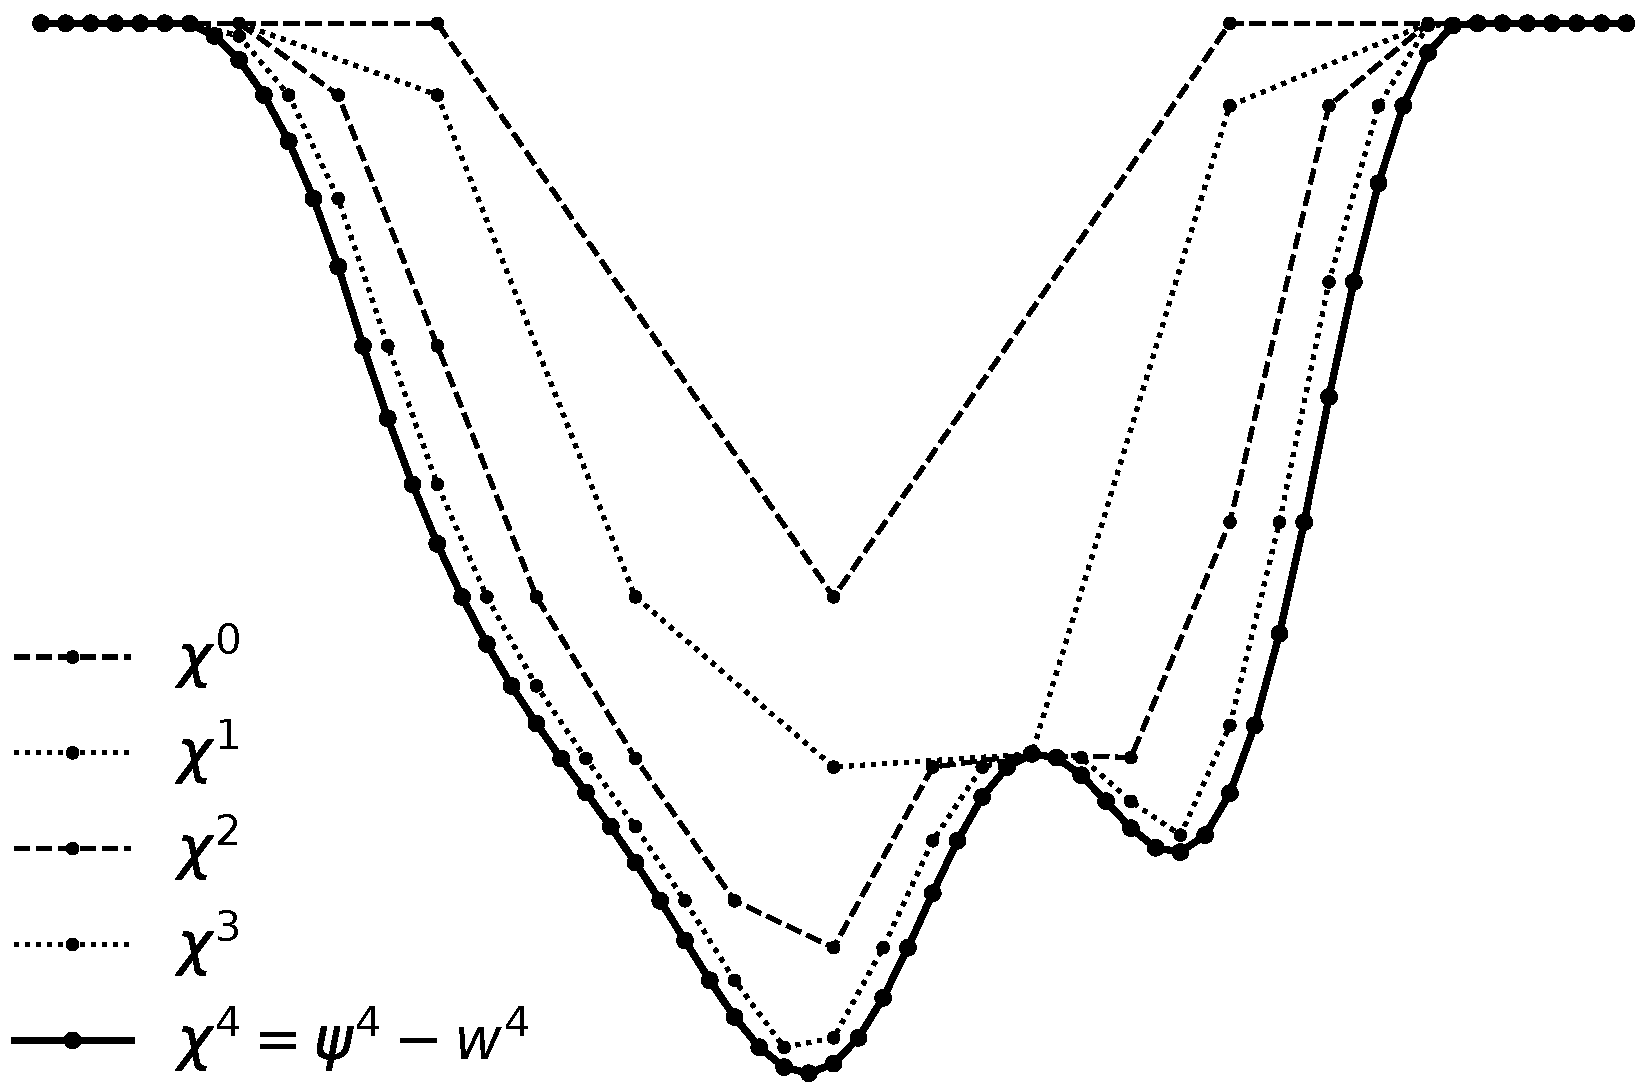
\includegraphics[width=0.65\textwidth]{fixfigs/chiphilevels.pdf}
\caption{The level defect constraints (LDC) $\underline{\chi}^j$ are generated from $\underline{\chi}^J = \underline{\gamma}^J - w^J$ using maximum restriction: $\underline{\chi}^j = \maxR \underline{\chi}^{j+1}$.}
\label{fig:chiphilevels}
\end{figure}

Intuitively-speaking, the LDC $\underline{\chi}^j$ is the most-negative function from $\tilde{\mathcal{V}}^j$ such that if another element of $\tilde{\mathcal{V}}^j$ is above $\underline{\chi}^j$ then it is also above $\underline{\chi}^{j+1}$, and similar comments apply to $\overline{\chi}^{j}$.  This construction of the box constraints on each coarser level is designed to permit the largest corrections from the coarsest levels \cite{GraeserKornhuber2009}, which promotes V-cycle efficiency.  Note that for the multilevel scheme in the following Sections, any system satisfying \eqref{eq:fe:chiordering} will suffice; the particular formulas in \eqref{eq:fe:chilevels} are not required when generating the LDCs $\underline{\chi}^{j},\overline{\chi}^{j}$.

We now compute the LDC differences:
\begin{equation}
\underline{\phi}^j = \underline{\chi}^j - \underline{\chi}^{j-1}, \qquad \overline{\phi}^j = \overline{\chi}^j - \overline{\chi}^{j-1}.  \label{eq:fe:philevels}
\end{equation}
We take $\underline{\chi}^{-1}=\overline{\chi}^{-1}=0$ so that $\underline{\phi}^0=\underline{\chi}^0$ and $\overline{\phi}^0=\overline{\chi}^0$.  Regarding subtraction of extended real-valued quantities, if $\underline{\chi}^j(x_p)=-\infty$ then we set $\underline{\phi}^j(x_p)=-\infty$ regardless of the value of $\underline{\chi}^{j-1}(x_p)$, and similarly $\overline{\phi}^j(x_p)=+\infty$ if $\overline{\chi}^j(x_p)=+\infty$.  These new LDCs $\underline{\phi}^{j},\overline{\phi}^{j} \in \tilde{\mathcal{V}}^J$ again bracket zero: $\underline{\phi}^j \le 0 \le \overline{\phi}^j$.  Though  they are not ordered as in \eqref{eq:fe:chiordering}, telescoping sums hold for any $j=0,1,\dots,J$:
\begin{equation}
\sum_{i=0}^j \underline{\phi}^i = \underline{\chi}^j, \qquad \sum_{i=0}^j \overline{\phi}^i = \overline{\chi}^j.  \label{eq:fe:telescoping}
\end{equation}
Table \ref{tab:ldcs} should help the reader keep track of our box-constrained LDC system.

\begin{table}[H]
\begin{tabular}{llc}
\emph{name}        & \emph{formulas} \\ \hline
(finest) upward & ${\Large \strut} \underline{\chi}^J = \underline{\gamma}^J - w^J,\quad \overline{\chi}^J = \overline{\gamma}^J - w^J$ \\
upward          & ${\Large \strut} \underline{\chi}^{j} = \maxR \underline{\chi}^{j+1}, \quad \overline{\chi}^{j} = \minR \overline{\chi}^{j+1}$ \\
downward        & ${\Large \strut} \underline{\phi}^j = \underline{\chi}^j - \underline{\chi}^{j-1}, \quad \overline{\phi}^j = \overline{\chi}^j - \overline{\chi}^{j-1}$
\end{tabular}

\medskip
\caption{Box level defect constraints (LDCs).}
\label{tab:ldcs}
\end{table}


\section{Multilevel CDs} \label{sec:cdmultilevel}

A multilevel V-cycle solver is defined in the next Section.  This V-cycle uses LDCs $\underline{\phi}^j,\overline{\phi}^j$ for the downward side and $\underline{\chi}^j,\overline{\chi}^j$ for the upward side.  The corresponding \emph{downward} and \emph{upward defect constraint sets}, respectively, are
\begin{align}
\mathcal{D}^j = \left\{v \in \mathcal{V}^j \,:\, \underline{\phi}^j \le v \le \overline{\phi}^j \text{ and } \, v|_{\partial_D\Omega} = 0\right\}, \label{eq:fe:constraintsets} \\
\mathcal{U}^j = \left\{v \in \mathcal{V}^j \,:\, \underline{\chi}^j \le v \le \overline{\chi}^j \text{ and } \, v|_{\partial_D\Omega} = 0\right\}. \notag
\end{align}
These are closed and convex subsets of the FE spaces $\mathcal{V}^j$.  Because $\underline{\chi}^j \le \underline{\phi}^j \le 0 \le \overline{\phi}^j \le \overline{\chi}^j$, it follows that $\mathcal{D}^j \subset \mathcal{U}^j$.  Note that the finest-level set $\mathcal{U}^J$ is equivalent to the original constraint set $\mathcal{K}^J$: for all $z^J \in \mathcal{V}^J$,
\begin{equation}
z^J \in \mathcal{U}^J \quad \iff \quad w^J+z^J \in \mathcal{K}^J. \label{eq:fe:finestlevelequivalent}
\end{equation}

Our multilevel strategy is based on incomplete constraint decompositions (CDs; Section \ref{sec:cd}) of $\mathcal{U}^J$, as we now explain.  Each upward set $\mathcal{U}^j$ can be decomposed in an inclusion sense, becoming a true CD in unilateral cases.  The following Lemma is based on the unilateral CD construction underlying Algorithm 4.7 in \cite{GraeserKornhuber2009}; see also equation (59) in \cite{Tai2003}.

\begin{lemma}  \label{lem:downwardadmissibility}  For arbitrary upper and lower obstacles $\underline{\gamma}^J,\overline{\gamma}^J$ satisfying \eqref{eq:fe:boxconstraintrequirements}, and $j=0,1,\dots,J$,
\begin{equation}
\mathcal{U}^j \supset \mathcal{D}^j + \mathcal{D}^{j-1} + \dots + \mathcal{D}^0. \label{eq:fe:downwardsuminclusion}
\end{equation}
In unilateral cases, where either $\underline{\gamma}^J=-\infty$ or $\overline{\gamma}^J=+\infty$, inclusion \eqref{eq:fe:downwardsuminclusion} becomes a full CD \eqref{eq:constraintdecomp}, namely $\mathcal{U}^j=\sum_{i=0}^j \mathcal{D}^i$.
\end{lemma}

\begin{proof}  Subspace decomposition \eqref{eq:subspacedecomp} holds---see nesting \eqref{eq:fe:nestedspaces}---and definition \eqref{eq:fe:constraintsets} shows $\mathcal{D}^i \subset \mathcal{U}^i \subset \cV^i$.  If $y^i \in \mathcal{D}^i$ for $0 \le i \le j$ then by \eqref{eq:fe:telescoping},
\begin{equation}
\underline{\chi}^j = \sum_{i=0}^j \underline{\phi}^i \le \sum_{i=0}^j y^i \le \sum_{i=0}^j \overline{\phi}^i \le \overline{\chi}^j \label{eq:fe:lemmaordering}
\end{equation}
thus \eqref{eq:fe:downwardsuminclusion} holds for any box constraints.

In unilateral cases we can also construct decomposition operators $\Pi_i$ and show \eqref{eq:constraintrestrictionsum}.  Suppose $\overline{\gamma}^J=+\infty$, thus $\overline{\chi}^j=+\infty$ and $\overline{\phi}^i = +\infty$ for all levels.  For $v\in \mathcal{V}^j$ and $0\le i \le j$, let $I_{j\to i}^\ominus$ be the operator applying the minimum (monotone) restriction $j-i$ times, mapping into $\mathcal{V}^i$:
\begin{equation}
I_{j\to i}^\ominus v = \minR(\dots(\minR v)\dots)  \label{eq:fe:minimummaps}
\end{equation}
Note that $I_{j\to j}^\ominus v = v$, and set $I_{j\to -1}^\ominus=0$ by definition.  From operators \eqref{eq:fe:minimummaps} we define the nonlinear decomposition operators $\Pi_i:\mathcal{U}^j \to \mathcal{D}^i$:
\begin{equation}
\Pi_i z^j = I_{j\to i}^\ominus(z^j - \underline{\chi}^j) - I_{j\to i-1}^\ominus(z^j - \underline{\chi}^j) + \underline{\phi}^i.  \label{eq:fe:unilateraldecompositionoperator}
\end{equation}
(Compare equation (4.9) in \cite{GraeserKornhuber2009}.)  Property \eqref{eq:fe:monotonerestrictionprops} implies $I_{j\to i}^\ominus(z^j - \underline{\chi}^j) \ge I_{j\to i-1}^\ominus(z^j - \underline{\chi}^j)$, thus $\Pi_i z^j \ge \underline{\phi}^i$, so $\Pi_i z^j \in \mathcal{D}^i$ (in this unilateral case).  On the other hand, the following sum telescopes, leaving only its first term plus the sum in \eqref{eq:fe:telescoping}:
\begin{align*}
\sum_{i=0}^j \Pi_i z^j &= z^j - \underline{\chi}^j + \sum_{i=0}^j \underline{\phi}^i = z^j.
\end{align*}
This shows \eqref{eq:constraintrestrictionsum}, thus that \eqref{eq:fe:downwardsuminclusion} is equality, a true CD \eqref{eq:constraintdecomp}.  The $\underline{\gamma}^J=-\infty$ case is similar.
\end{proof}

It is tempting to try to turn \eqref{eq:fe:downwardsuminclusion} into a full CD for arbitrary box constraints by using decomposition maps like $\Pi_i$.  Specifically, one might split $z^j = \min\{z^j,0\} + \max\{z^j,0\}$ and apply unilateral formulas like \eqref{eq:fe:unilateraldecompositionoperator} to $\min\{z^j,0\}$ and $\max\{z^j,0\}$ separately, with $\Pi_i$ applied to $\min\{z^j,0\}$ and a straightforward variant operator to $\max\{z^j,0\}$.  In fact, the lower bound $\Pi_i (\min\{z^j,0\}) \ge \underline{\phi}^i$ holds, as shown in the above proof.  However, the following Example shows why $\Pi_i(\min\{z^j,0\})$ may have an arbitrarily large maximum, and thus exceed any finite upper LDC $\overline{\phi}^i$, so unfortunately $\Pi_i$ does not map even non-positive functions to $\mathcal{D}^i$ in the presence of a finite upper LDC.  On the other hand, the existence of an entirely-different strategy for showing a full CD is not excluded.

\begin{example}  \label{ex:notfullcd}
Let $a\ge 0$ be an arbitrary positive number.  Consider a 2-level hierarchy ($J=1$), and suppose the lower defect constraint is the constant function $\underline{\chi}^1=-a$.  Recalling Table \ref{tab:ldcs}, note $\underline{\chi}^0=\maxR \underline{\chi}^1=-a$ also, so $\underline{\phi}^1=0$ and $\underline{\phi}^0=-a$.  Suppose $z^1$ is a ``sawtooth'' function which takes on value $-a$ on the coarse nodes and value $0$ on the other fine-level nodes.  Then $\overline{\chi}^1 \ge 0 \ge z^1\ge \underline{\chi}^1$, for any valid $\overline{\chi}^1$, so $z^j \in \mathcal{U}^1$.  However, $I_{1\to 0}^\ominus(z^1 - \underline{\chi}^1) = \minR(z^1 - \underline{\chi}^1) = 0$ identically.  From \eqref{eq:fe:unilateraldecompositionoperator}, $\Pi_1 z^1$ simplifies to $\Pi_1 z^1 = z^1 - \underline{\chi}^1$.  But then $\Pi_1 z^1$ attains a maximum $a\ge 0$.  This maximum can be chosen to exceed any upper defect obstacle $\overline{\phi}^1$.  Thus, for general $w^1 \in \mathcal{U}^1$ and general LDCs, $\Pi_1$ does not map $\min\{w^1,0\}$ into $\mathcal{D}^1$.
\end{example}

Each upward defect constraint set $\mathcal{U}^j$ can also be be decomposed down to an arbitrary level $k$ where an upward set $\mathcal{U}^k$ is used as the coarsest set.  While similar to Lemma \ref{lem:downwardadmissibility}, the next Lemma does not follow logically from it.

\begin{lemma}  \label{lem:upwardadmissibility}  For any $j=0,1,\dots,J$ and $0\le k\le j$,
\begin{equation}
\mathcal{U}^j \supseteq \mathcal{D}^j + \mathcal{D}^{j-1} + \dots + \mathcal{D}^{k+1} + \mathcal{U}^k \label{eq:fe:upwardsuminclusion}
\end{equation}
In unilateral cases, where either $\underline{\gamma}^J=-\infty$ or $\overline{\gamma}^J=+\infty$, inclusion \eqref{eq:fe:upwardsuminclusion} is a full CD \eqref{eq:constraintdecomp}. \end{lemma}

\begin{proof}  Definition \eqref{eq:fe:philevels} shows that $\underline{\chi}^j = \underline{\phi}^j + \dots + \underline{\phi}^{k+1} + \underline{\chi}^k$ and $\overline{\chi}^j = \overline{\phi}^j + \dots + \overline{\phi}^{k+1} + \overline{\chi}^k$.  (These facts replace \eqref{eq:fe:telescoping}.)  If $y^i \in \mathcal{D}^i$ for $k+1 \le i \le j$ and $z^k \in \mathcal{U}^k$ then it is easy to show, as in \eqref{eq:fe:lemmaordering}, that $\underline{\chi}^j \le y^j + \dots + y^{k+1} + z^k \le \overline{\chi}^j$, thus \eqref{eq:fe:upwardsuminclusion} holds.

In unilateral cases we follow the proof of Lemma \ref{lem:downwardadmissibility}.  Definition \eqref{eq:fe:minimummaps} is unchanged.  We can use \eqref{eq:fe:unilateraldecompositionoperator} unchanged for $i=k+1,\dots,j$, but it must be modified in the $i=k$ case: $\Pi_k z^j = I_{j\to k}^\ominus(z^j - \underline{\chi}^j) + \underline{\chi}^k$.  The remainder of the proof goes through as for Lemma \ref{lem:downwardadmissibility}.
\end{proof}

In summary, inclusions \eqref{eq:fe:downwardsuminclusion} and \eqref{eq:fe:upwardsuminclusion} suffice to show the admissibility of all iterates and corrections in V-cycle Algorithm \ref{alg:fascd}.  Lemma \ref{lem:downwardadmissibility} explains downward admissibility, and Lemma \ref{lem:upwardadmissibility} upward admissibility, in Algorithm \ref{alg:fascd}.  However, a convergence analysis following \cite{Tai2003} or \cite{GraeserKornhuber2009}, somehow extending their arguments to VIs \eqref{eq:vi} which are not of minimization type, and/or to box constraints, would seem to require full CDs, and perhaps new ideas.


\section{Full approximation storage constraint decomposition (\fascd) V-cycle} \label{sec:vcycle}

The \fascd V-cycle algorithm in this section uses Lemmas \ref{lem:downwardadmissibility} and \ref{lem:upwardadmissibility}, that is, it smooths in $\mathcal{D}^j$ and $\mathcal{U}^j$ during the downward and upward stages, respectively.  \fascd extends the multilevel CD schemes of Tai \cite{Tai2003} and Gr\"aser \& Kornhuber \cite[Algorithm 4.7]{GraeserKornhuber2009} by following a nonlinear FAS approach \cite{BrandtLivne2011}, and in fact it reduces to FAS for PDEs when inequality constraints are removed (Appendix \ref{app:reductions}).

The V-cycle generates a correction to a finest-level iterate $w^J \in \mathcal{K}^J$ based on perturbations from each coarser FE subspace $\mathcal{V}^j$.  By nesting \eqref{eq:fe:nestedspaces} these corrections also live in the fine-level subspace $\mathcal{V}^J$, but we will use prolongation $P$ to indicate where the computer representation changes.  Note that we coarsen both the residual and the solution iterate, in constrast to classical linear multigrid wherein only the residual is coarsened.

However, the corrected iterate needs to be admissible.  In detail, suppose $y^i \in \mathcal{D}^i$ for $i=J,\dots,j-1$ are already-computed corrections during the downward part of the V-cycle (Figure \ref{fig:fascdvcycle}).  By \eqref{eq:fe:downwardsuminclusion} the correction at this point is admissible, namely $y^J + \dots + y^{j+1} \in \mathcal{U}^J$, equivalently $w^J + y^J + \dots + y^{j+1} \in \mathcal{K}^J$.  Smoothing, an incomplete solution process on a VI problem (Section \ref{sec:smoothers}), then occurs at the next-coarser level, yielding the next correction $y^j \in \mathcal{D}^j$.  At the bottom the coarsest-level VI is then solved (also Section \ref{sec:smoothers}), resulting in the full downward correction $y^J + \dots + y^1 + z^0 \in \mathcal{U}^J$.  Starting upward, $y^1 + z^0 \in \mathcal{U}^1$ is an initial iterate for smoothing on level $j=1$.  Smoothing in $\mathcal{U}^1$ yields admissible correction $y^J + \dots + y^2 + z^1 \in \mathcal{U}^J$ using \eqref{eq:fe:upwardsuminclusion}.  Continuing in this ``telescoping'' way, up-smoothing in the constraint sets $\mathcal{U}^j$, starting from initial iterate $y^j+z^{j-1}$, finally generates $z^J\in \mathcal{U}^J$ as the full V-cycle correction.  Then the next admissible iterate is $w^J + z^J \in \mathcal{K}^J$.

\begin{figure}[ht]
\begin{center}
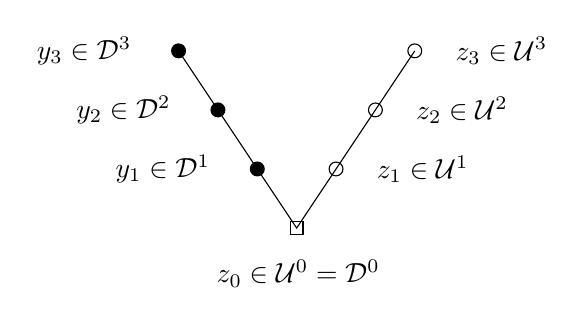
\begin{tikzpicture}[scale=1.0]
  \pgfmathsetmacro\hstep{0.5}
  \pgfmathsetmacro\vstep{0.75}
  \pgfmathsetmacro\ceps{0.08}   % size of square for coarse grid

% V-cycle with MCD down-obstacle and up-obstacle annotations
  \draw[black,thin] (-\hstep,3*\vstep) -- (0.0,2*\vstep) -- (\hstep,\vstep) --  (2*\hstep,0.0)
                    -- (3*\hstep,\vstep) -- (4*\hstep,2*\vstep) -- (5*\hstep,3*\vstep);
  \filldraw (-\hstep,3*\vstep) node[xshift=-12mm] {$y_3 \in \mathcal{D}^3$} circle (2.5pt);
  \filldraw (0.0,2*\vstep) node[xshift=-12mm] {$y_2 \in \mathcal{D}^2$} circle (2.5pt);
  \filldraw (\hstep,\vstep) node[xshift=-12mm] {$y_1 \in \mathcal{D}^1$} circle (2.5pt);
  \draw     (2*\hstep-\ceps,-\ceps) node[xshift=1mm,yshift=-5mm] {$z_0 \in \mathcal{U}^0 = \mathcal{D}^0$} rectangle (2*\hstep+\ceps,+\ceps);
  \draw     (3*\hstep,\vstep) node[xshift=11mm] {$z_1 \in \mathcal{U}^1$} circle (2.5pt);
  \draw     (4*\hstep,2*\vstep) node[xshift=11mm] {$z_2 \in \mathcal{U}^2$} circle (2.5pt);
  \draw     (5*\hstep,3*\vstep) node[xshift=11mm] {$z_3 \in \mathcal{U}^3$} circle (2.5pt);
\end{tikzpicture}

\end{center}
\caption{The \fascd V-cycle computes downward corrections $y_j \in \mathcal{D}^j$, but the upward corrections $z_j\in\mathcal{U}^j$ are in larger sets.}
\label{fig:fascdvcycle}
\end{figure}

A key idea is that, because $\mathcal{U}^j\supset \mathcal{D}^j$, up-smoothing solves less-restricted VI problems than down-smoothing.  Intuitively-speaking, going downward one does not know what the upcoming coarse corrections will be, so they must be in the sufficiently-small sets $\mathcal{D}^j$ so that their sum is admissible once we return to a level.  However, going upward no further \emph{coarser} corrections, relative to that level, can violate admissibility.

To state \fascd Algorithm \ref{alg:fascd} below we must clarify the problems solved at each mesh level.  As in FAS multigrid for nonlinear PDEs \cite{BrandtLivne2011,Bruneetal2015,Trottenbergetal2001}, both the solution approximation and the residual must be coarsened, and a source functional created.  On mesh level $j$ we assume a re-discretized nonlinear operator $f^j$, with output in $(\cV^j)'$, which is an FE discretization of $f$ in \eqref{eq:boxdirichletvi}, presumably using quadrature and etc.~in the same scheme which generated $f^J$ in \eqref{eq:fe:vi}.  Note that finest-level problem \eqref{eq:fe:vi} uses the original source functional $\ell^J$, and an admissible iterate $w^J \in \mathcal{K}^J$ has already\footnote{Conceptually-speaking this is true.  In practice the LDCs $\underline{\chi}^j,\overline{\chi}^j,\underline{\phi}^j,\overline{\phi}^j$ are generated during the descent stage; see Algorithm \ref{alg:fascd}.  Observe that the LDCs do not depend on $w^j$ for $j<J$, nor on the corrections $y^j,z^j$.} been used to general the LDCs and constraint sets $\mathcal{D}^j$, $\mathcal{U}^j$ at each level (Section \ref{sec:ldcs}).

As we descend $j<J$, we define new $j$th-level iterates
\begin{equation}
w^j = \iR(w^{j+1} + y^{j+1}),  \label{eq:fe:definew}
\end{equation}
the value \emph{before} smoothing and/or correction at level $j$.  From $w^j$ we define $\ell^j \in (\cV^j)'$:
\begin{equation}
\ell^j = \begin{cases} \ell^J, & j=J \\
                       f^j(w^j) + R\left(\ell^{j+1}-f^{j+1}(w^{j+1}+y^{j+1})\right), & j<J. \end{cases} \label{eq:fe:levelsource}
\end{equation}
Observe that injection $\iR$ coarsens the iterates---injection is commonly used in classical FAS \cite[section 5.3]{Trottenbergetal2001}---while canonical restriction $R$ coarsens linear functionals.  (Recall Table \ref{tab:transfers} summarizes our transfer operators.)

On descent, at levels $j=J,J-1,\dots,1$, we solve the following VI for $y^j \in \mathcal{D}^j$:
\begin{equation}
\ip{f^j(w^j + y^j)}{v-y^j} \ge \ip{\ell^j}{v-y^j} \qquad \text{for all } v\in \mathcal{D}^j, \label{eq:fe:downvi}
\end{equation}
for which the initial iterate is $y_{(0)}^j=0$.  (Zero is admissible; see the comment after \eqref{eq:fe:philevels}.)  On ascent, $j=0,1,\dots,J$, the same VI is solved, but in a larger admissible set, for $z^j \in \mathcal{U}^j$:
\begin{equation}
\ip{f^j(w^j + z^j)}{v-z^j} \ge \ip{\ell^j}{v-z^j} \qquad \text{for all } v\in \mathcal{U}^j. \label{eq:fe:upvi}
\end{equation}
The nontrivial initial iterate for this problem is found by prolonging the coarser-level correction $z^{j-1}$, and using it to correct the current (down-smoothed) correction on the level,\footnote{Prolongation $P$ is used in \eqref{eq:fe:upwardinitial} to reflect the change in FE representation, from $\mathcal{V}^{j-1}$ to $\mathcal{V}^{j}$.}
\begin{equation}
z_{(0)}^j = y^j + P z^{j-1},  \label{eq:fe:upwardinitial}
\end{equation}
but with $z_{(0)}^0=0$ on the coarsest level.  Note $z_{(0)}^j$ is admissible since $\mathcal{D}^j + \mathcal{U}^{j-1} \subset \mathcal{U}^j$; see \eqref{eq:fe:upwardsuminclusion}.

If we were to inject the original box constraints \eqref{eq:fe:fineconstraintset} downward to coarser meshes, i.e.~$\underline{\gamma}^j = \iR \underline{\gamma}^{j+1}$ and $\overline{\gamma}^j = \iR \overline{\gamma}^{j+1}$, then, because injection preserves inequalities, and because $y^{j+1} \in \mathcal{D}^{j+1}$, it would follow from \eqref{eq:fe:definew} that $\underline{\gamma}^j \le w^j \le \overline{\gamma}^j$.  In this sense $w^j$ is admissible with respect to the box constraints, but, following \cite{GraeserKornhuber2009}, our use of LDCs (Table \ref{tab:ldcs}) avoids the need to generate such box constraints $\underline{\gamma}^j$ and $\overline{\gamma}^j$ on each level.  (Note that while $w^j \in \cV^j \subset \cV^J$ holds, generally $w^j \notin \cK^J$.)  In any case, Algorithm \ref{alg:fascd} will yield a final, finest-level iterate $w^J+z^J \in \cK^J$ which is genuinely admissible for problem \eqref{eq:fe:vi}.

Regarding formula \eqref{eq:fe:levelsource}, the formula for source functional $\ell^j$ is a classical FAS construction.  (Compare equation (8.5b) in \cite{BrandtLivne2011} or equation (5.3.14) in \cite{Trottenbergetal2001}.)  It has the following explanation, mimicking the PDE version, which simultaneously justifies \eqref{eq:fe:levelsource} and VI problems \eqref{eq:fe:downvi} and \eqref{eq:fe:upvi}.  First, the $j+1$ level problem \eqref{eq:fe:downvi} is not solved exactly by the finer-level correction $y^{j+1}$---the down-smoother was only approximate---so we seek a further correction $y$ on the $j+1$ level so that
\begin{equation}
\ip{f^{j+1}(w^{j+1}+y^{j+1}+y)}{v-y^{j+1}-y} \ge \ip{\ell^{j+1}}{v-y^{j+1}-y} \quad \text{\emph{(notional)}} \label{eq:fe:downvinotional}
\end{equation}
for all $v\in \mathcal{D}^j$.  However, $y$ will actually be approximated from solving a coarser, $j$th-level problem generated by modifying \eqref{eq:fe:downvinotional} in 4 steps:
\begin{enumerate}
\item subtract the computable quantity $f^{j+1}(w^{j+1}+y^{j+1}) \in (\mathcal{V}^{j+1})'$ from both sides,
\item replace the residual $\ell^{j+1}-f^{j+1}(w^{j+1}+y^{j+1})$ on the right by its restriction,
\item replace $w^{j+1}+y^{j+1}$, where it appears on the left, by its restriction,
\item and, where it appears on the left, replace $f^{j+1}$ by the coarser rediscretization $f^j$.
\end{enumerate}
Steps \emph{(ii)}--\emph{(iv)} are justified when the residual and the error are smooth as a result of the progress made by the $j+1$ level down-smoother \cite[subsection 5.3.4, for example]{Trottenbergetal2001}.  These steps now yield a problem for the $j$th-level correction $y^j \in \mathcal{D}^j$:
\begin{align}
&\ip{f^j\left(\iR(w^{j+1}+y^{j+1})+y^j\right)}{v-y^j} - \ip{f^j\left(\iR(w^{j+1}+y^{j+1})\right)}{v-y^j} \label{eq:fe:downvicluttered} \\
&\qquad \ge \ip{R\left(\ell^{j+1}-f^{j+1}(w^{j+1}+y^{j+1})\right)}{v-y^j} \notag
\end{align}
This is the same as VI problem \eqref{eq:fe:downvi}, but in cluttered form; definitions \eqref{eq:fe:definew} and \eqref{eq:fe:levelsource} yields \eqref{eq:fe:downvi}.  The explanation for VI \eqref{eq:fe:upvi} is essentially identical.

We will regard the smoothers for VI problems \eqref{eq:fe:downvi} and \eqref{eq:fe:upvi} as approximate, in-place procedures, acting on the corrections $y^j$ and $z^j$, respectively (Section \ref{sec:smoothers}).  Also, as is standard in multigrid, at the coarsest $j=0$ level we suppose that problem \eqref{eq:fe:upvi} is solved quite accurately.  However, this coarsest-level solver may be the same as the other smoothers, perhaps with a stronger tolerance.

These ideas come together in Algorithm \ref{alg:fascd}.  \pr{fascd-vcycle} acts in-place on $w^J$, and it assumes certain semantics for the \pr{smooth} and the coarsest-level \pr{solve} procedures (Section \ref{sec:smoothers}).  These do in-place modifications of their final arguments, without modifying their first four arguments.  $\pr{smooth}^{\id{down}}$ and $\pr{smooth}^{\id{up}}$ denote \id{down} and \id{up} iterations, respectively.

\begin{pseudofloat}[ht]
\begin{pseudo}
\pr{fascd-vcycle}(\ell^J,\underline{\gamma}^J,\overline{\gamma}^J;w^J)\text{:} \\+
    $\underline{\chi}^J = \underline{\gamma}^J - w^J {\large \strut}$ \\
    $\overline{\chi}^J = \overline{\gamma}^J - w^J {\large \strut}$ \\
    for $j=J$ downto $j=1$ \\+
      $\underline{\chi}^{j-1} = \maxR \underline{\chi}^j {\large \strut}$ \\
      $\overline{\chi}^{j-1} = \minR \overline{\chi}^j {\large \strut}$ \\
      $\underline{\phi}^j = \underline{\chi}^j - P\underline{\chi}^{j-1} {\large \strut}$ \\
      $\overline{\phi}^j = \overline{\chi}^j - P\overline{\chi}^{j-1} {\large \strut}$ \\
      $y^j = 0$ \\
      $\text{\pr{smooth}}^{\text{\id{down}}}(\ell^j,\underline{\phi}^j,\overline{\phi}^j,w^j;y^j)$  \ct{smoothing of \eqref{eq:fe:downvi} in $\mathcal{D}^j$}\\
      $w^{j-1} = \iR(w^j + y^j)$ \\
      $\ell^{j-1} = f^{j-1}(w^{j-1}) + R \left(\ell^j - f^j(w^j+y^j)\right)$ \\-
    $z^0 = 0$ \\
    $\text{\pr{solve}}(\ell^0,\underline{\chi}^0,\overline{\chi}^0,w^0;z^0)$ \hspace{1.0cm} \ct{solving of \eqref{eq:fe:upvi} in $\mathcal{U}^0$} \\
    for $j=1$ to $j=J$ \\+
      $z^j = y^{j} + P z^{j-1}$ \\
      $\text{\pr{smooth}}^{\text{\id{up}}}(\ell^j,\underline{\chi}^j,\overline{\chi}^j,w^j;z^j)$  \ct{smoothing of \eqref{eq:fe:upvi} in $\mathcal{U}^j$} \\-
    $w^J \gets w^J+z^J$
\end{pseudo}
\caption{The \fascd V-cycle as an iteration for solving FE VI problem \eqref{eq:fe:vi}.  $f^j$ denotes an FE discretization of $f$ in problem \eqref{eq:boxdirichletvi}.}
\label{alg:fascd}
\end{pseudofloat}

Regarding storage required for \pr{fascd-vcycle}, and assuming all box constraints are nontrivial, 7 vectors must be allocated on each level: $\underline{\chi}^j$, $\overline{\chi}^j$, $\underline{\phi}^j$, $\overline{\phi}^j$, $w^j$, $\ell^j$, $y^j$.  Note $z^j$ can use the same storage as $y^j$.  On the finest level one must also store $\underline{\gamma}^J$ and $\overline{\gamma}^J$, while on the coarsest level there are only 5 vectors because $\underline{\phi}^0=\underline{\chi}^0$ and $\overline{\phi}^0=\overline{\chi}^0$.  Therefore, using standard estimates for 2D refinement plus a geometric series argument \cite{Trottenbergetal2001}, the total floating-point storage, excluding the implementations of smoothers and the coarse-level solver, is
\begin{equation}
9 m_J + 7 m_{J-1} + \dots + 7 m_1 + 5 m_0 \approx \left(9 + 7 \sum_{k=1}^\infty \frac{1}{4^k}\right) m_J \approx 11 m_J.
\end{equation}
For comparison, a single-level method needs $4 m_J$ storage for the vectors $\underline{\gamma}^J,\overline{\gamma}^J,\ell^J,w^J$.

If some of the obstacles are trivial, for instance if $\overline{\gamma}^J=+\infty$ in a unilateral obstacle problem, storage is correspondingly reduced at all levels.  Furthermore, we will see in Section \ref{sec:results} that, though \pr{fascd-vcycle} defines a general $V(\pr{down},\pr{up})$ cycle for VI problems, in fact the $V(0,\pr{up})$ case generally produces the best performance.  In that case the storage is reduced to about $9 m_J$ by neglecting the downward LDCs $\underline{\phi}^j$, $\overline{\phi}^j$ at all levels.

Repeated application of \pr{fascd-vcycle} to solve VI \eqref{eq:fe:vi} will not reduce the finest-level residual $f^J(w^J) - \ell^J$ to zero everywhere because the problem is inequality-constrained.  We need to identify the vector quantity whose norm must be controlled by a tolerance.  Recalling mixed complementarity problem \eqref{eq:fe:mcp}, and denoting the hat function at node $x_p \in \mathcal{T}^J$ by $\psi_p$, for $w^J \in \mathcal{K}^J$ we define the finest-level \emph{nodal complementarity residual} in $\RR^{m_J}$.  It is defined in the four cases listed after \ref{eq:fe:mcp}, namely inactive, lower active, upper active, and boundary:
\begin{equation}
\hat r(w^J)_p = \begin{cases}
    \ip{f^J(w^J)-\ell^J}{\psi_p}, & \underline{\gamma}^J(x_p) < w^J(x_p) < \overline{\gamma}^J(x_p), \\
    \min\{\ip{f^J(w^J)-\ell^J}{\psi_p},0\}, & w^J(x_p) = \underline{\gamma}^J(x_p), \\
    \max\{\ip{f^J(w^J)-\ell^J}{\psi_p},0\}, & w^J(x_p) = \overline{\gamma}^J(x_p), \\
    w^J(x_p) - g_D^J(x_p), & x_p \in \partial_D\Omega. \end{cases} \label{eq:cpresidual}
\end{equation}
Where the box constraints pinch at $x_p \notin \partial_D\Omega$, i.e.~where $\underline{\gamma}^J(x_p)=u^J(x_p)=\overline{\gamma}^J(x_p)$, we define $\hat r(w^J)_p=0$.  Note that $\hat r:\mathcal{V}^J \to \RR^{m_J}$ is a computable nonlinear map derived from $f^J$ and the vectors $\ell^J$, $\underline{\gamma}^J$, and $\overline{\gamma}^J$.  For unconstrained PDEs one would use only the inactive and boundary cases.

The idea here is that $\hat r(w^J)$ is nonzero only if there are nodes where MCP \eqref{eq:fe:mcp} is violated, either because the pointwise residual $\ip{f^J(w^J)-\ell^J}{\psi_p}$ remains nonzero where the constraints are inactive, or because it has the wrong sign on an actively-constrained degree of freedom, or because the Dirichlet boundary condition is not satisfied.

A solver for \eqref{eq:fe:vi} using repeated applications of \pr{fascd-vcycle} would start with an initial iterate $w_{(0)}^J$, do V-cycles, and stop once the finest-level nodal residual $\hat r(w^J)$ was sufficiently small.  For example, using tolerances \id{atol}$>0$ and \id{rtol}$>0$ the stopping criterion might be
\begin{equation}
\|\hat r(w^J)\| < \id{atol} \qquad \text{or} \qquad \frac{\|\hat r(w^J)\|}{\|\hat r((w^J)^{(0)})\|} < \id{rtol},
\end{equation}
for some norm $\|\cdot\|$ on $\RR^{m_J}$.  A step tolerance could also be used, measuring the difference between successive iterates.


\section{Smoother implementations} \label{sec:smoothers}

FIXME  Recall that a $j$th-level hat function based at node $x_p^j$ is denoted $\psi_p^j$, for an iterate $g^j$ and an admissible correction $y^j \in \mathcal{D}^j$ we define the \emph{downward nodal residual} as
\begin{equation}
(\hat r_{\text{down}}(y^j))_p = \begin{cases} \ip{f^j(g^j+y^j)-\ell^j}{\psi_p^j}, & y^j(x_p^j) > \phi^j(x_p^j), \\
                                  \min\{\ip{f^j(g^j+y^j)-\ell^j}{\psi_p^j},0\}, & y^j(x_p^j) = \phi^j(x_p^j). \end{cases} \label{eq:dncpresidual}
\end{equation}
The \emph{upward nodal residual} $\hat r_{\text{up}}(z^j)$ for $z^j \in \mathcal{U}^j$ is similarly defined using $\chi^j$.

FIXME stopping criteria for smoother


\section{Results and discussion} \label{sec:results}

FIXME show results for 2D Firedrake implementation of FASCD for $p$-Laplacian obstacle problem (Example \ref{ex:plaplacian}), advection-diffusion obstacle problem (Example \ref{ex:advectiondiffusion}), and porous-media obstacle problem (Example \ref{ex:porous})

FIXME observe that up-smoothing is more efficient; this observation seems to be new; compare the comments on V(1,0) and V(1,1) cycles in \cite{GraeserKornhuber2009,Tai2003}

FIXME constrast the implemented examples in \cite{GraeserKornhuber2009,Tai2003} in which $f$ is linear


% A BRIDGE TOO FAR:  \section{Results for a nonlocal variational inequality}


\bibliography{fascd}
\bibliographystyle{siam}


\appendix
\section{Reductions of FASCD to familiar multilevel algorithms} \label{app:reductions}

Algorithm \ref{alg:fascd} in the main text, \pr{fascd-vcycle}, generalizes two better-known multilevel algorithms.  First we show that it reduces to the FAS multigrid V-cycle for nonlinear PDEs (which itself generalizes the standard linear multigrid V-cycle \cite{Trottenbergetal2001}).  Second we reduce FASCD to an existing MCD V-cycle for unilateral linear variational inequalities \cite{GraeserKornhuber2009}.  This Appendix helps readers understand Algorithm \ref{alg:fascd} by separating those assumptions which relate to nonlinear and FAS aspects from the nontrivial modifications of standard multigrid which are caused by inequality constraints.  The later arise even when $f$ in \eqref{eq:vi} is a linear operator.

To derive the classical FAS multigrid V-cycle from Algorithm \ref{alg:fascd}, we remove the inequality constraints from VI problem \eqref{eq:fe:vi} and then simplify the pseudocode accordingly.  To do this we suppose that the finest-level obstacles $\underline{\gamma}^J$ and $\overline{\gamma}^J$ are very negative and positive, respectively, with magnitude exceeding $u^J$ or any prospective iterate $w^J$.  Finest-level problem \eqref{eq:fe:vi} is then unconstrained except for its Dirichlet boundary conditions.  Let $\mathcal{V}_0^J \subset \mathcal{V}^J$ denote the space with zero values on $\partial_D\Omega$.  By replacing ``$v-u^J$'' with an arbitrary $v \in \mathcal{V}_0^J$ we have the finest-level, weak form problem
\begin{equation}
\ip{f^J(u^J)}{v} = \ip{\ell^J}{v} \qquad \text{for all } v\in \mathcal{V}_0^J \label{eq:app:fas:pde}
\end{equation}
corresponding to the strong-form PDE $f(u)=\ell$.

Furthermore, the downward $\mathcal{D}^j$ and upward $\mathcal{U}^j$ constraint sets can be arbitrarily enlarged so that the coarser-level corrections $y^j$ and $z^j$ in Algorithm \ref{alg:fascd} are also never constrained.  Formally-speaking we might do this, still satisfying the LDC ordering property \eqref{eq:fe:chiordering}, by choosing LDCs with all gaps being large so that $\underline{\chi}^j \ll 0 \ll \overline{\chi}^j$ and also $\underline{\phi}^j = \underline{\chi}^j - \underline{\chi}^{j-1} \ll 0 \ll \overline{\phi}^j = \overline{\chi}^j - \overline{\chi}^{j-1}$.\footnote{As noted after \eqref{eq:fe:chiordering}, the application of monotone restriction operators $\maxR,\minR$ is not required to generate LDCs $\underline{\chi}^j$ and $\overline{\chi}^j$ satisfying the ordering property.}

Now the correction VIs \eqref{eq:fe:downvi} and \eqref{eq:fe:upvi} are also unconstrained, and lines 2--3 and 6--9 can be removed from Algorithm \ref{alg:fascd}.  Also, because the downward corrections $y^j$ are no longer separately constrained, we may simply refer to the corrected solution $w^j=g^j+y^j$ instead of $g^j$ and $y^j$ separately.  Then the smoothers and the coarsest-level solver can be regarded as in-place modifications of $w^j$.  Now noting $g^{j-1}=\iR w^j$ in line 12, after down-smoothing, the coarsened source functional can be rewritten using notation $w^{j-1}=\iR w^j$:
\begin{equation}
\ell^{j-1} = f^{j-1}\left(w^{j-1}\right) + R\left(\ell^j-f^j(w^j)\right). \label{eq:app:fas:levelsource}
\end{equation}
(Compare line 13 of Algorithm \ref{alg:fascd}.)

At the completion of down-smoothing the solution iterate on the $j$th level is $w^j=g^j+y^j$.  Now we must be careful that going upward only the coarse correction, and not the coarse solution, gets prolonged.\footnote{Compare Remark 5.3.9 in \cite{Trottenbergetal2001}, a warning to novices.}  The coarser-level iterate is $w^{j-1} = g^{j-1}+z^{j-1}$ after up-smoothing on the $j-1$ level.  From Algorithm \ref{alg:fascd} the initial value of the correction $z^j$, before smoothing, is $z^j = y^j + P z^{j-1}$.  These facts imply that the $j$th-level iterate before up-smoothing must be set to
    $$w^j \gets w^j + Pz^j = (g^j+y^j)+P(w^{j-1} - g^{j-1}) = w^j + P(w^{j-1} - \iR w^j).$$
This is a standard FAS statement.  In fact, with the given modifications, we have the much-simplified pseudocode in Algorithm \ref{alg:fas}.  This FAS V-cycle algorithm appears in various places, for example Algorithm 14 of \cite{Bruneetal2015} or in section 5.3.4 of \cite{Trottenbergetal2001}.

\begin{pseudofloat}[ht]
\begin{pseudo} \label{ps:fas-vcycle}
\pr{fas-vcycle}(\ell^J; w^J)\text{:} \\+
    for $j=J$ downto $j=1$ \\+
      $\text{\pr{smooth}}^{\text{\id{down}}}(\ell^j;w^j)$ \\
      $w^{j-1} = \iR w^j$ \\
      $\ell^{j-1} = f^{j-1}(w^{j-1}) + R \left(\ell^j - f^j(w^j)\right)$ \\-
    $\text{\pr{solve}}(\ell^0;w^0)$ \\
    for $j=1$ to $j=J$ \\+
      $w^j \gets w^j + P (w^{j-1} - \iR w^j)$ \\
      $\text{\pr{smooth}}^{\text{\id{up}}}(\ell^j;w^j)$ \\-
\end{pseudo}
\caption{An FAS V-cycle results from removing the inequality constraints from \pr{fascd-vcycle}, and simplifying accordingly.}
\label{alg:fas}
\end{pseudofloat}

FIXME by assuming $f$ is linear, reduce to Algorithm 4.7 in \cite{GraeserKornhuber2009} but with $\text{V}(\nu_1,\nu_2)$ cycles

\end{document}
